% =====================================================================
% COMP3111 F2026 - Activity 1 - HKUST Marketplace
% Class diagram, use-case diagram and use-case specifications.
%
% Compile with pdflatex (twice), e.g.  latexmk -pdf main.tex
% or upload the whole folder to Overleaf (compiler: pdfLaTeX).
%
% Files:  main.tex          cover, class diagram, use-case diagram, index
%         specs_buyer.tex   3.1 Task 1 (Buyer)  - to be written by Person A
%         specs_seller.tex  3.2 Task 2 (Seller) - done
%         specs_admin.tex   3.3 Task 3 (Admin)  - to be written by Person C
%         figures/          all diagrams (vector PDF), incl. one small
%                           diagram per use case for all 28 use cases
% =====================================================================
\documentclass[10pt,a4paper]{article}

\usepackage[T1]{fontenc}
\usepackage[utf8]{inputenc}
\usepackage[scaled=0.95]{helvet}
\renewcommand{\familydefault}{\sfdefault}
\usepackage[a4paper,top=17mm,bottom=20mm,left=18mm,right=18mm]{geometry}
\usepackage[table]{xcolor}
\usepackage{graphicx,array,tabularx,multicol,enumitem,fancyhdr,tcolorbox}
\usepackage[hidelinks]{hyperref}

% ---------------------------------------------------------------------
% TEAM INFORMATION: replace the values below (used on the cover and in
% the task allocation). Remove \fillin{...} once a value is filled in.
% ---------------------------------------------------------------------
\newcommand{\fillin}[1]{\colorbox{fillyellow}{\strut #1}}
\newcommand{\GroupName}{HKUST Marketplace Group}
\newcommand{\NameA}{Charles DUPOUY}   \newcommand{\IdA}{21431599}   \newcommand{\EmailA}{cerdupouy@connect.ust.hk}   % Task 1 Buyer
\newcommand{\NameB}{Antoine LEPIN}    \newcommand{\IdB}{21431678}   \newcommand{\EmailB}{alepin@connect.ust.hk}      % Task 2 Seller
\newcommand{\NameC}{Elio Le Dortz}    \newcommand{\IdC}{21431666}   \newcommand{\EmailC}{eledortz@connect.ust.hk}    % Task 3 Admin

% ---------------------------------------------------------------------
% Style (colours of the course's use-case specification template)
% ---------------------------------------------------------------------
\definecolor{ucred}{HTML}{B0001E}
\definecolor{epblue}{HTML}{1F3BD6}
\definecolor{fillyellow}{HTML}{FFF3A6}
\definecolor{headpink}{HTML}{F3E6E8}
\definecolor{rowgray}{HTML}{F2F2F2}

\setlength{\parindent}{0pt}
\setlength{\parskip}{2pt}
\linespread{1.1}
\setlist{nosep,leftmargin=1.4em}

\pagestyle{fancy}
\fancyhf{}
\renewcommand{\headrulewidth}{0pt}
\fancyfoot[L]{\footnotesize\color{gray}\thepage}
\fancyfoot[R]{\footnotesize\color{gray}COMP3111 F2026 \textperiodcentered{} Activity 1 \textperiodcentered{} HKUST Marketplace}

% Section heading: large title with a red rule under it
\newcommand{\sectionhead}[1]{%
  {\fontsize{16}{19}\selectfont\bfseries #1\par}\vspace{-2pt}%
  {\color{ucred}\rule{\linewidth}{1.2pt}}\par\vspace{5pt}}

% ---- Use-case specification commands ----
% \usecase{Name}{Task}  : new page + "Use Case: Name"
\newcommand{\usecasetitle}[2]{%
  {\color{ucred}\fontsize{14}{17}\selectfont\bfseries\underline{Use Case: #1}}%
  \hspace{8pt}{\small\color{gray}Task #2}\par\vspace{2pt}}
\newcommand{\usecase}[2]{\clearpage\usecasetitle{#1}{#2}}
% Section of a specification (Brief Description, Basic Flow, ...)
\newcommand{\ucsec}[1]{\par\vspace{7pt}{\color{ucred}\large\bfseries #1}\par\nopagebreak\vspace{1pt}}
% Small use-case diagram from figures/
\newcommand{\ucdiagram}[1]{\par\includegraphics[height=27mm]{figures/#1}\par}
% Extension point {Name}: inline, on its own line, or indented one level
\newcommand{\ep}[1]{\textcolor{epblue}{\textbf{\{#1\}}}}
\newcommand{\eppoint}[1]{\par\vspace{2pt}\ep{#1}\par\nopagebreak}
\newcommand{\eppointi}[1]{\par\vspace{2pt}\hspace*{2.2em}\ep{#1}\par\nopagebreak}
% Name of a subflow when it is called ("Perform subflow ...")
\newcommand{\subflowref}[1]{\textcolor{ucred}{\textbf{\textit{#1}}}}
% Numbered steps: \st (1.), \sti (3.1.), \stii (3.1.1.)
\newcommand{\st}[2]{\par\hangindent=1.9em\hangafter=1\makebox[1.9em][l]{#1}#2\par}
\newcommand{\sti}[2]{\par\hangindent=5em\hangafter=1\hspace*{2.2em}\makebox[2.8em][l]{#1}#2\par}
\newcommand{\stii}[2]{\par\hangindent=8em\hangafter=1\hspace*{4.4em}\makebox[3.6em][l]{#1}#2\par}
% Subflow (S1: ...) or alternative flow (A1: ...), kept on one page
\newenvironment{flowblock}[1]%
  {\par\vspace{6pt}\noindent\begin{minipage}{\linewidth}\setlength{\parskip}{2pt}%
   {\color{ucred}\bfseries\itshape #1}\par}%
  {\end{minipage}\par}
% Yellow box for parts that still have to be written
\newtcolorbox{todobox}{colback=yellow!12,colframe=yellow!55!black,boxrule=0.8pt,arc=0pt,left=6pt,right=6pt}

\begin{document}

% =====================================================================
% Cover
% =====================================================================
\thispagestyle{fancy}
\begin{center}
  \vspace*{4mm}
  {\color{darkgray}COMP3111 Software Engineering \textperiodcentered{} Fall 2026}\par\vspace{7mm}
  {\color{ucred}\fontsize{30}{34}\selectfont\bfseries Activity 1}\par\vspace{3mm}
  {\fontsize{20}{24}\selectfont\bfseries HKUST Marketplace}\par\vspace{3mm}
  {\color{darkgray}Class Diagram \textperiodcentered{} Use-Case Diagram \textperiodcentered{} Use-Case Specifications}
\end{center}
\vspace{6mm}

{\color{ucred}\large\bfseries Team Information}\par\vspace{3pt}
\renewcommand{\arraystretch}{1.35}
\begin{tabularx}{\linewidth}{|p{0.22\linewidth}|p{0.17\linewidth}|X|p{0.22\linewidth}|}\hline
\cellcolor{headpink}\textbf{Group} & \multicolumn{3}{l|}{\GroupName}\\\hline
\rowcolor{headpink}\textbf{Member} & \textbf{Student ID} & \textbf{Email} & \textbf{Main task}\\\hline
\NameA & \IdA & \EmailA & Task 1: Buyer Portal\\\hline
\NameB & \IdB & \EmailB & Task 2: Seller Portal\\\hline
\NameC & \IdC & \EmailC & Task 3: Admin Portal\\\hline
\end{tabularx}

\vspace{6mm}
{\color{ucred}\large\bfseries Task Allocation}\par\vspace{3pt}
\begin{tabularx}{\linewidth}{|X|p{0.26\linewidth}|p{0.14\linewidth}|}\hline
\rowcolor{headpink}\textbf{Part of this document} & \textbf{Responsible} & \textbf{Score}\\\hline
1. Class diagram & Whole team & Team\\\hline
2. Use-case diagram & Whole team & Team\\\hline
3.1 Use-case specifications, Task 1: Buyer Portal (11 use cases) & \NameA & Individual\\\hline
3.2 Use-case specifications, Task 2: Seller Portal (9 use cases) & \NameB & Individual\\\hline
3.3 Use-case specifications, Task 3: Admin Portal (8 use cases) & \NameC & Individual\\\hline
\end{tabularx}
\renewcommand{\arraystretch}{1}

\vspace{6mm}
{\color{ucred}\large\bfseries Contents}\par\vspace{3pt}
1. Class Diagram\par
2. Use-Case Diagram\par
3. Use-Case Specifications\par
\hspace*{1.5em}3.1 Task 1: Buyer Portal\par
\hspace*{1.5em}3.2 Task 2: Seller Portal\par
\hspace*{1.5em}3.3 Task 3: Admin Portal\par
\vspace{5mm}
{\small\color{darkgray}All use-case specifications follow Style 2 (with subflows) of the course's use-case detailed specification template.}

% =====================================================================
% 1. Class Diagram
% =====================================================================
\clearpage
\sectionhead{1. Class Diagram}
13 classes. User is abstract; Buyer, Seller and Admin are its disjoint and complete subclasses.\par\vspace{3pt}
\begin{center}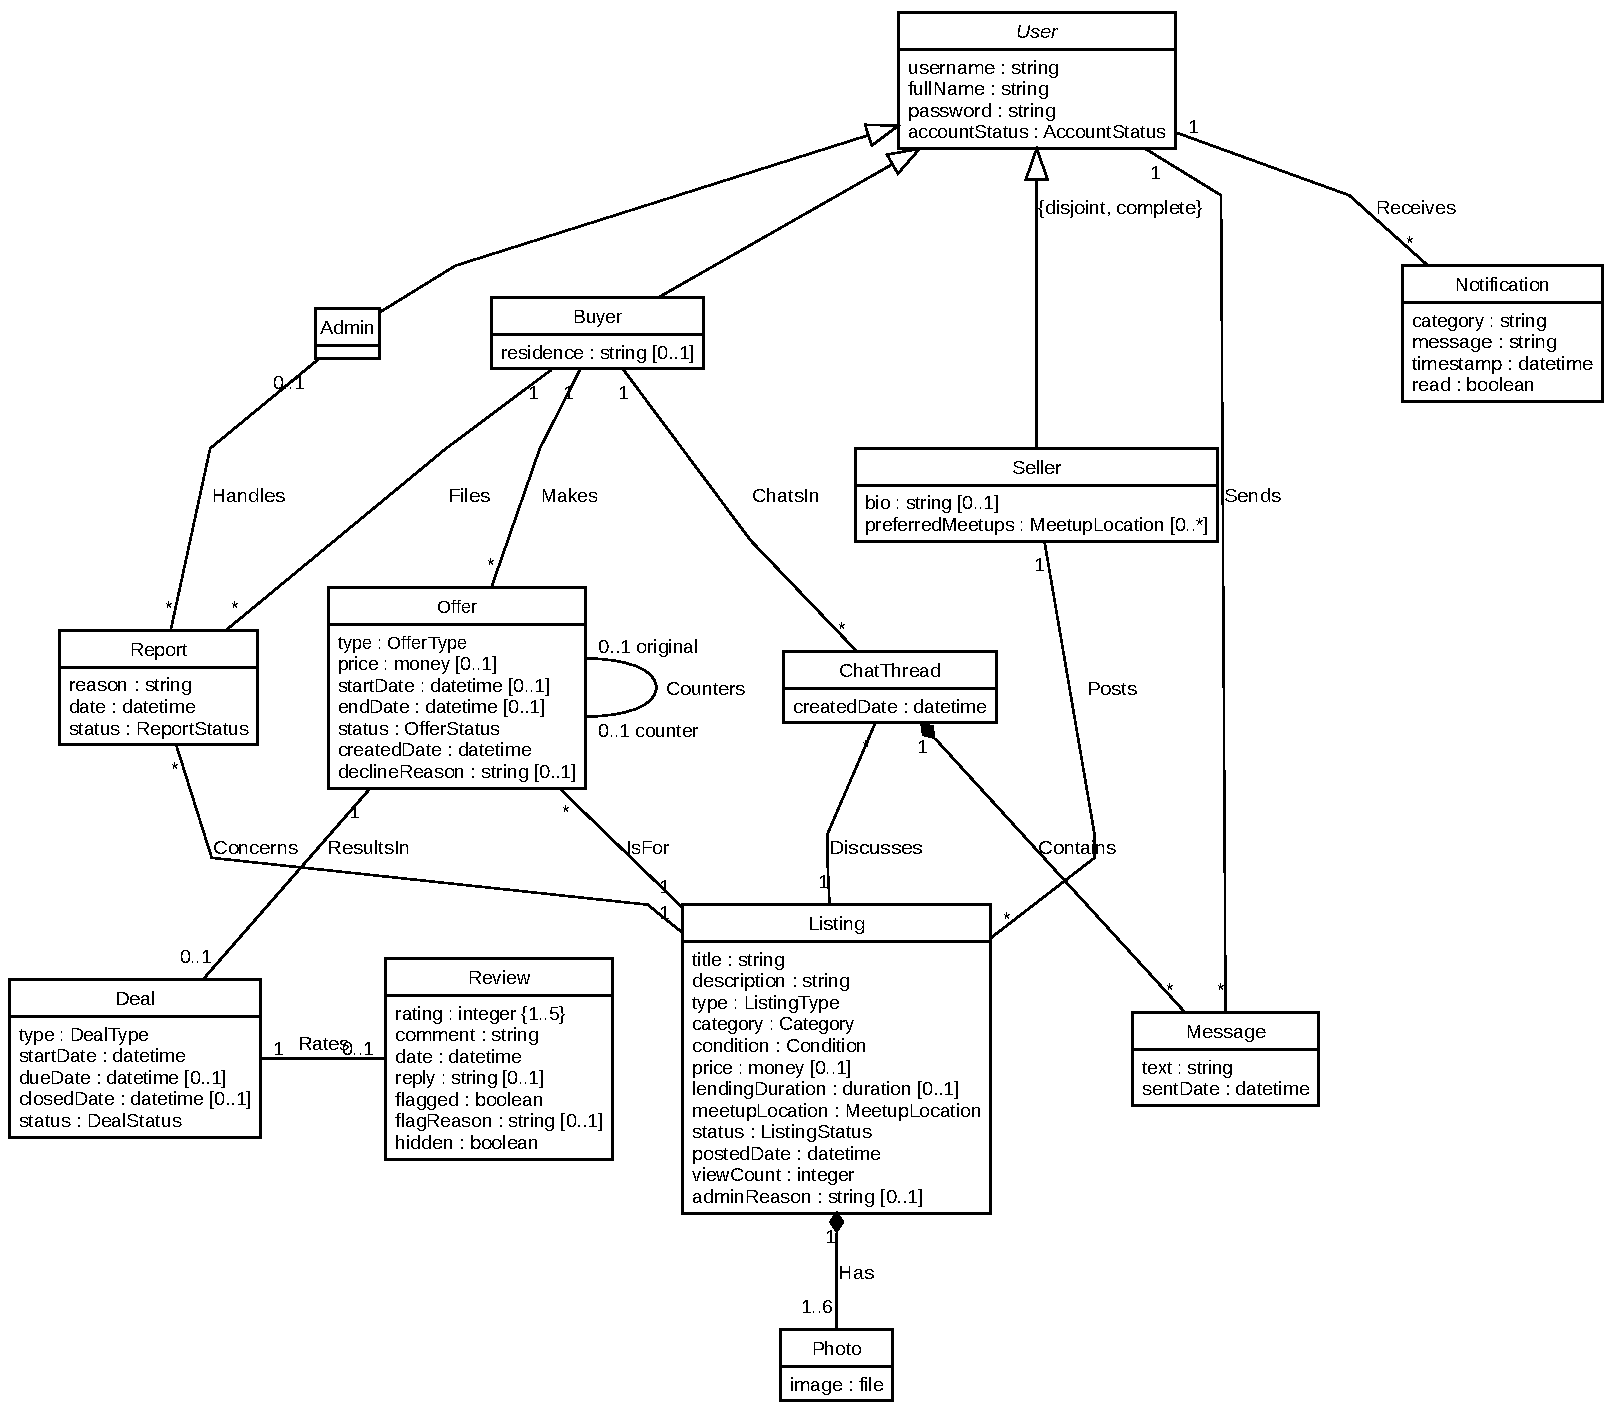
\includegraphics[width=0.93\linewidth]{figures/class_diagram}\end{center}\vspace{-8pt}

\ucsec{Enumerations}
{\footnotesize\renewcommand{\arraystretch}{1.05}\noindent
\begin{tabular}[t]{|l|}\hline\multicolumn{1}{|c|}{\tiny\guillemotleft{}enumeration\guillemotright{}}\\[-2pt]\multicolumn{1}{|c|}{\textbf{AccountStatus}}\\\hline Active\\ Deactivated\\ Deleted\\\hline\end{tabular}\hfill \begin{tabular}[t]{|l|}\hline\multicolumn{1}{|c|}{\tiny\guillemotleft{}enumeration\guillemotright{}}\\[-2pt]\multicolumn{1}{|c|}{\textbf{ListingType}}\\\hline Sell\\ Lend\\ GiveAway\\\hline\end{tabular}\hfill \begin{tabular}[t]{|l|}\hline\multicolumn{1}{|c|}{\tiny\guillemotleft{}enumeration\guillemotright{}}\\[-2pt]\multicolumn{1}{|c|}{\textbf{ListingStatus}}\\\hline PendingReview\\ Live\\ Rejected\\ Reserved\\ Sold\\ Lent\\ Given\\ Removed\\\hline\end{tabular}\hfill \begin{tabular}[t]{|l|}\hline\multicolumn{1}{|c|}{\tiny\guillemotleft{}enumeration\guillemotright{}}\\[-2pt]\multicolumn{1}{|c|}{\textbf{Category}}\\\hline Books\\ Electronics\\ Furniture\\ Clothing\\ Stationery\\ Sports\\ Other\\\hline\end{tabular}\hfill \begin{tabular}[t]{|l|}\hline\multicolumn{1}{|c|}{\tiny\guillemotleft{}enumeration\guillemotright{}}\\[-2pt]\multicolumn{1}{|c|}{\textbf{Condition}}\\\hline New\\ LikeNew\\ Used\\ ForParts\\\hline\end{tabular}\hfill \begin{tabular}[t]{|l|}\hline\multicolumn{1}{|c|}{\tiny\guillemotleft{}enumeration\guillemotright{}}\\[-2pt]\multicolumn{1}{|c|}{\textbf{MeetupLocation}}\\\hline Atrium\\ Library\\ LG1Canteen\\ LG7Canteen\\ NorthGate\\ SouthGate\\ StudentHalls\\\hline\end{tabular}

\medskip\noindent
\begin{tabular}[t]{|l|}\hline\multicolumn{1}{|c|}{\tiny\guillemotleft{}enumeration\guillemotright{}}\\[-2pt]\multicolumn{1}{|c|}{\textbf{OfferType}}\\\hline PriceOffer\\ BorrowRequest\\ Claim\\\hline\end{tabular}\hfill \begin{tabular}[t]{|l|}\hline\multicolumn{1}{|c|}{\tiny\guillemotleft{}enumeration\guillemotright{}}\\[-2pt]\multicolumn{1}{|c|}{\textbf{OfferStatus}}\\\hline Pending\\ Accepted\\ Declined\\ Countered\\ Withdrawn\\\hline\end{tabular}\hfill \begin{tabular}[t]{|l|}\hline\multicolumn{1}{|c|}{\tiny\guillemotleft{}enumeration\guillemotright{}}\\[-2pt]\multicolumn{1}{|c|}{\textbf{DealType}}\\\hline Sale\\ Loan\\ Giveaway\\\hline\end{tabular}\hfill \begin{tabular}[t]{|l|}\hline\multicolumn{1}{|c|}{\tiny\guillemotleft{}enumeration\guillemotright{}}\\[-2pt]\multicolumn{1}{|c|}{\textbf{DealStatus}}\\\hline Active\\ Completed\\ Returned\\\hline\end{tabular}\hfill \begin{tabular}[t]{|l|}\hline\multicolumn{1}{|c|}{\tiny\guillemotleft{}enumeration\guillemotright{}}\\[-2pt]\multicolumn{1}{|c|}{\textbf{ReportStatus}}\\\hline Open\\ Resolved\\\hline\end{tabular}\hfill\mbox{}
}

\vspace{3mm}
{\small
\begin{itemize}
  \item Following Lecture 6, object identifiers and get/set operations are not shown.
  \item A counter offer is an Offer linked to the original offer through Counters (roles original and counter).
  \item Deleted users and listings are kept with status Deleted or Removed (soft delete), so deals, chats and reviews keep their history.
\end{itemize}}

% =====================================================================
% 2. Use-Case Diagram
% =====================================================================
\clearpage
\sectionhead{2. Use-Case Diagram}
The HKUST Marketplace has 3 actors and 28 use cases. Chat About Listing is the only use case shared by two actors (Buyer and Seller).\par
\begin{center}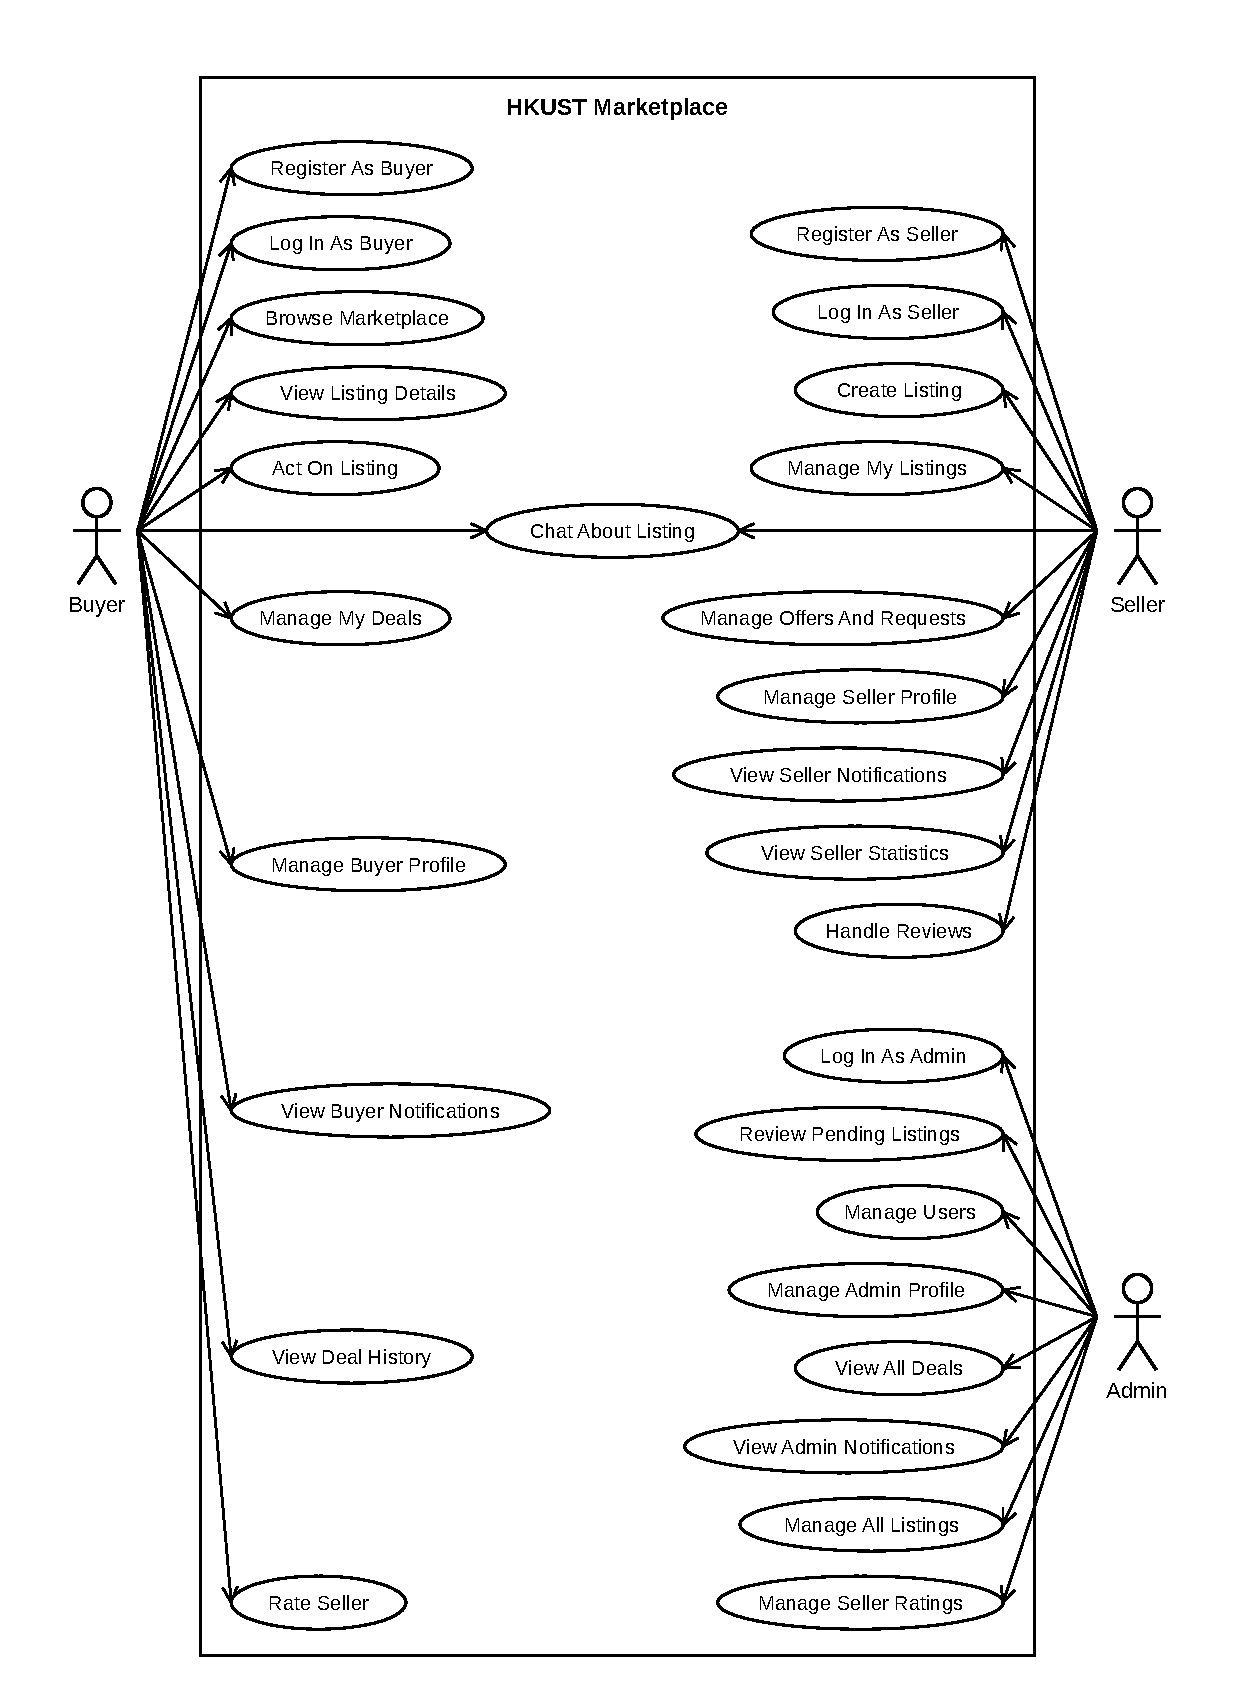
\includegraphics[height=0.70\textheight]{figures/usecase_diagram_team}\end{center}
{\small\renewcommand{\arraystretch}{1.3}
\begin{tabularx}{\linewidth}{|p{0.12\linewidth}|X|}\hline
\rowcolor{headpink}\textbf{Actor} & \textbf{Description}\\\hline
Buyer & A student or staff member who browses listings and buys, borrows or claims items through the Buyer Portal.\\\hline
Seller & A student or staff member who posts items to sell, lend or give away, and handles the offers received, through the Seller Portal.\\\hline
Admin & A staff member who moderates listings, users and ratings through the Admin Portal, using a seeded account (no registration).\\\hline
\end{tabularx}}

% =====================================================================
% 3. Use-Case Specifications
% =====================================================================
\clearpage
\sectionhead{3. Use-Case Specifications}
One specification is written for each use case in the diagram. The table maps each use case to its project subtask.\par\vspace{4pt}
{\small\renewcommand{\arraystretch}{1.15}
\begin{tabularx}{\linewidth}{|X|p{0.14\linewidth}|p{0.2\linewidth}|}\hline
\rowcolor{headpink}\textbf{Use case} & \textbf{Subtask} & \textbf{Actor(s)}\\\hline
\rowcolor{rowgray}\multicolumn{3}{|l|}{\textbf{Task 1: Buyer Portal}}\\\hline
Register As Buyer & 1.1 & Buyer\\\hline
Log In As Buyer & 1.2 & Buyer\\\hline
Browse Marketplace & 1.3 & Buyer\\\hline
View Listing Details & 1.4 & Buyer\\\hline
Act On Listing & 1.5 & Buyer\\\hline
Chat About Listing & 1.5 & Buyer, Seller\\\hline
Manage My Deals & 1.6 & Buyer\\\hline
Manage Buyer Profile & 1.7 & Buyer\\\hline
View Buyer Notifications & 1.8 & Buyer\\\hline
View Deal History & 1.9 & Buyer\\\hline
Rate Seller & 1.10 & Buyer\\\hline
\rowcolor{rowgray}\multicolumn{3}{|l|}{\textbf{Task 2: Seller Portal}}\\\hline
Register As Seller & 2.1 & Seller\\\hline
Log In As Seller & 2.2 & Seller\\\hline
Create Listing & 2.3 & Seller\\\hline
Manage My Listings & 2.4 & Seller\\\hline
Manage Offers And Requests & 2.5 & Seller\\\hline
Manage Seller Profile & 2.6 & Seller\\\hline
View Seller Notifications & 2.7 & Seller\\\hline
View Seller Statistics & 2.8 & Seller\\\hline
Handle Reviews & 2.9 & Seller\\\hline
\rowcolor{rowgray}\multicolumn{3}{|l|}{\textbf{Task 3: Admin Portal}}\\\hline
Log In As Admin & 3.1 & Admin\\\hline
Review Pending Listings & 3.2 & Admin\\\hline
Manage Users & 3.3 & Admin\\\hline
Manage Admin Profile & 3.4 & Admin\\\hline
View All Deals & 3.5 & Admin\\\hline
View Admin Notifications & 3.6 & Admin\\\hline
Manage All Listings & 3.7 & Admin\\\hline
Manage Seller Ratings & 3.8 & Admin\\\hline
\end{tabularx}}

% =====================================================================
% 3.1 Task 1: Buyer Portal  (11 use-case specifications, Style 2)
% =====================================================================

% ---------------------------------------------------------------------
\clearpage
\sectionhead{3.1 Task 1: Buyer Portal}
\usecasetitle{Register As Buyer}{1.1}
\ucsec{Brief Description}
This use case describes how a student or staff member creates a Buyer account so that they can browse listings and make offers.\par
\ucsec{Use-case Diagram}
\ucdiagram{uc_Register_As_Buyer}
\ucsec{Basic Flow}
\st{1.}{The use case begins when the Buyer actor chooses to register a buyer account.}
\st{2.}{The system displays the buyer registration form.}
\eppoint{Enter Details}
\st{3.}{The Buyer enters a username, full name, password and confirm password, and optionally a residence hall or off-campus location.}
\eppoint{Submit Registration}
\st{4.}{The Buyer submits the form.}
\eppoint{Validate Details}
\st{5.}{The system checks that the username is unique across all buyer, seller and admin accounts, the full name is not empty, the password meets the password rules, and the confirm password matches the password.}
\st{6.}{The system creates the Buyer account, storing the password in hashed form.}
\st{7.}{The system informs the Buyer that the registration succeeded and displays the Buyer login screen.}
\st{8.}{The use case ends.}
\ucsec{Postconditions}
If the use case ends successfully, a new Buyer account is stored and can be used to log in to the Buyer Portal.\par
\ucsec{Alternative Flows}
\begin{flowblock}{A1: Duplicate Username}
At \ep{Validate Details} if the username is already used by any buyer, seller or admin account,\par
\st{1.}{The system informs the Buyer that the username is already taken.}
\st{2.}{The flow of events is resumed at \ep{Enter Details}.}
\end{flowblock}
\begin{flowblock}{A2: Empty Required Field}
At \ep{Validate Details} if the username, full name or password is empty,\par
\st{1.}{The system highlights the empty fields.}
\st{2.}{The flow of events is resumed at \ep{Enter Details}.}
\end{flowblock}
\begin{flowblock}{A3: Weak Password}
At \ep{Validate Details} if the password does not meet the password rules,\par
\st{1.}{The system informs the Buyer which password rules are not met.}
\st{2.}{The flow of events is resumed at \ep{Enter Details}.}
\end{flowblock}
\begin{flowblock}{A4: Passwords Do Not Match}
At \ep{Validate Details} if the confirm password does not match the password,\par
\st{1.}{The system informs the Buyer that the passwords do not match.}
\st{2.}{The flow of events is resumed at \ep{Enter Details}.}
\end{flowblock}
\begin{flowblock}{A5: Cancel Registration}
At any point between \ep{Enter Details} and \ep{Submit Registration},\par
\st{1.}{The Buyer can cancel the registration.}
\st{2.}{The use case ends and no account is created.}
\end{flowblock}
\ucsec{Special Requirements}
\begin{itemize}
  \item Passwords are stored hashed, never in plaintext.
  \item Password rules: at least 8 characters, with at least one uppercase letter, one lowercase letter and one digit.
\end{itemize}

% ---------------------------------------------------------------------
\usecase{Log In As Buyer}{1.2}
\ucsec{Brief Description}
This use case describes how a registered Buyer logs in to access the Buyer Portal.\par
\ucsec{Use-case Diagram}
\ucdiagram{uc_Log_In_As_Buyer}
\ucsec{Basic Flow}
\st{1.}{The use case begins when the Buyer actor chooses to log in to the Buyer Portal.}
\st{2.}{The system displays the login screen.}
\eppoint{Enter Credentials}
\st{3.}{The Buyer enters a username and password and submits them.}
\eppoint{Validate Credentials}
\st{4.}{The system checks the username and password against the registered user accounts.}
\eppoint{Check Account Type}
\st{5.}{The system checks that the account is an active Buyer account.}
\st{6.}{The system starts a Buyer session and displays the Buyer dashboard.}
\st{7.}{The use case ends.}
\ucsec{Alternative Flows}
\begin{flowblock}{A1: Empty Field}
At \ep{Validate Credentials} if the username or password is empty,\par
\st{1.}{The system informs the Buyer that both fields are required.}
\st{2.}{The flow of events is resumed at \ep{Enter Credentials}.}
\end{flowblock}
\begin{flowblock}{A2: Invalid Credentials}
At \ep{Validate Credentials} if the username does not exist or the password is incorrect,\par
\st{1.}{The system informs the Buyer that the username or password is incorrect, without saying which one.}
\st{2.}{The flow of events is resumed at \ep{Enter Credentials}.}
\end{flowblock}
\begin{flowblock}{A3: Wrong Account Type}
At \ep{Check Account Type} if the account is a seller or admin account,\par
\st{1.}{The system informs the user that this account cannot log in to the Buyer Portal and must use its own portal.}
\st{2.}{The flow of events is resumed at \ep{Enter Credentials}.}
\end{flowblock}
\begin{flowblock}{A4: Account Deactivated}
At \ep{Check Account Type} if the Buyer account has been deactivated by the admin,\par
\st{1.}{The system informs the Buyer that the account is deactivated.}
\st{2.}{The use case ends.}
\end{flowblock}
\ucsec{Special Requirements}
\begin{itemize}
  \item Every Buyer-only function checks the Buyer session on the server side, so a seller or admin session cannot call it even without the user interface.
\end{itemize}

% ---------------------------------------------------------------------
\usecase{Browse Marketplace}{1.3}
\ucsec{Brief Description}
This use case describes how a Buyer browses, searches and filters the list of live listings available on the marketplace.\par
\ucsec{Use-case Diagram}
\ucdiagram{uc_Browse_Marketplace}
\ucsec{Preconditions}
The Buyer is logged in.\par
\ucsec{Basic Flow}
\st{1.}{The use case begins when the Buyer actor chooses to browse the marketplace.}
\st{2.}{The system retrieves all listings with status Live and displays them, each showing the title, seller name, category, listing type (Sell / Lend / GiveAway), price (if type is Sell), condition, meet-up location, posted date, availability status and thumbnail photo.}
\eppoint{Select Activity}
\st{3.}{While the Buyer has an activity to perform}
\sti{3.1.}{If SEARCH is selected}
\stii{3.1.1.}{Perform subflow \subflowref{Search Listings}.}
\sti{3.2.}{If FILTER is selected}
\stii{3.2.1.}{Perform subflow \subflowref{Filter Listings}.}
\sti{3.3.}{If SORT is selected}
\stii{3.3.1.}{Perform subflow \subflowref{Sort Listings}.}
\st{4.}{The use case ends.}
\ucsec{Subflows}
\begin{flowblock}{S1: Search Listings}
\eppoint{Enter Search Query}
\st{1.}{The Buyer enters a keyword or title.}
\eppoint{Apply Search}
\st{2.}{The system displays all Live listings whose title or description contain the keyword.}
\end{flowblock}
\begin{flowblock}{S2: Filter Listings}
\eppoint{Enter Filter Criteria}
\st{1.}{The Buyer selects one or more filter criteria: category, listing type, price range or condition.}
\eppoint{Apply Filter}
\st{2.}{The system displays all Live listings that match all the selected criteria.}
\end{flowblock}
\begin{flowblock}{S3: Sort Listings}
\eppoint{Select Sort Order}
\st{1.}{The Buyer selects a sort order: newest first, price low-to-high or price high-to-low.}
\eppoint{Apply Sort}
\st{2.}{The system redisplays the current listing results in the selected order.}
\end{flowblock}
\ucsec{Alternative Flows}
\begin{flowblock}{A1: No Listings Match}
At \ep{Apply Search} or \ep{Apply Filter} if no Live listings match the query or criteria,\par
\st{1.}{The system informs the Buyer that no listings match and displays an empty list.}
\st{2.}{The flow of events is resumed at \ep{Select Activity}.}
\end{flowblock}
\begin{flowblock}{A2: No Live Listings}
At the initial display in step 2 if there are no Live listings at all,\par
\st{1.}{The system informs the Buyer that there are no listings available yet.}
\st{2.}{The use case ends.}
\end{flowblock}

% ---------------------------------------------------------------------
\usecase{View Listing Details}{1.4}
\ucsec{Brief Description}
This use case describes how a Buyer opens a listing's detail page to see all its information, the seller's identity and average rating, and the available action buttons.\par
\ucsec{Use-case Diagram}
\ucdiagram{uc_View_Listing_Details}
\ucsec{Preconditions}
The Buyer is logged in.\par
\ucsec{Basic Flow}
\st{1.}{The use case begins when the Buyer actor selects a listing from the Browse Marketplace screen or from the My Deals screen.}
\st{2.}{The system increments the listing's view count.}
\st{3.}{The system displays the listing's full details: all photos (up to 6), title, full description, category, listing type, condition, meet-up location, posted date, availability status, price (Sell listings), lending duration (Lend listings), seller name and the seller's average rating.}
\st{4.}{The system displays the action button appropriate to the listing type: Make Offer (Sell), Borrow Request (Lend) or Claim (GiveAway), as well as a Chat button and a Report Listing button.}
\st{5.}{The use case ends.}
\ucsec{Alternative Flows}
\begin{flowblock}{A1: Listing No Longer Live}
At step 1 if the listing's status is no longer Live (for example it has been Reserved, Removed or Rejected after the Buyer navigated to it),\par
\st{1.}{The system informs the Buyer that the listing is no longer available.}
\st{2.}{The use case ends.}
\end{flowblock}
\begin{flowblock}{A2: Seller Has No Rating}
At step 3 if the seller has not yet received any rating,\par
\st{1.}{The system displays ``No ratings yet'' in place of the seller's average rating.}
\st{2.}{The flow of events is resumed at step 4.}
\end{flowblock}
\begin{flowblock}{A3: Report Listing}
At step 4 if the Buyer selects Report Listing,\par
\st{1.}{The system displays a form asking for a written reason.}
\st{2.}{The Buyer enters the reason and submits the report.}
\st{3.}{The system stores the report with status Open and notifies the admin.}
\st{4.}{The system confirms to the Buyer that the report has been submitted.}
\st{5.}{The use case ends.}
\end{flowblock}

% ---------------------------------------------------------------------
\usecase{Act On Listing}{1.5}
\ucsec{Brief Description}
This use case describes how a Buyer acts on a listing by submitting a price offer on a Sell listing, a borrow request on a Lend listing, or a claim on a GiveAway listing.\par
\ucsec{Use-case Diagram}
\ucdiagram{uc_Act_On_Listing}
\ucsec{Preconditions}
The Buyer is logged in and is viewing the Listing Detail screen.\par
\ucsec{Basic Flow}
\st{1.}{The use case begins when the Buyer actor selects an action button on the Listing Detail screen.}
\eppoint{Check Availability}
\st{2.}{The system checks that the listing is still Live.}
\eppoint{Select Action}
\st{3.}{If the listing type is Sell}
\sti{3.1.}{Perform subflow \subflowref{Submit Price Offer}.}
\st{4.}{If the listing type is Lend}
\sti{4.1.}{Perform subflow \subflowref{Submit Borrow Request}.}
\st{5.}{If the listing type is GiveAway}
\sti{5.1.}{Perform subflow \subflowref{Claim Item}.}
\st{6.}{The use case ends.}
\ucsec{Subflows}
\begin{flowblock}{S1: Submit Price Offer}
\eppoint{Enter Offer Price}
\st{1.}{The Buyer enters a proposed price.}
\eppoint{Confirm Offer}
\st{2.}{The Buyer submits the offer.}
\eppoint{Validate Offer}
\st{3.}{The system checks that the proposed price is a positive amount.}
\st{4.}{The system stores the offer with status Pending and notifies the seller.}
\st{5.}{The system confirms to the Buyer that the offer has been submitted.}
\end{flowblock}
\begin{flowblock}{S2: Submit Borrow Request}
\eppoint{Enter Borrow Dates}
\st{1.}{The Buyer enters a proposed start date and end date for the borrow period.}
\eppoint{Confirm Borrow Request}
\st{2.}{The Buyer submits the borrow request.}
\eppoint{Validate Borrow Request}
\st{3.}{The system checks that the start date is not in the past, the end date is after the start date, and the borrow period is at least 5 seconds.}
\st{4.}{The system stores the borrow request as an Offer with status Pending and notifies the seller.}
\st{5.}{The system confirms to the Buyer that the borrow request has been submitted.}
\end{flowblock}
\begin{flowblock}{S3: Claim Item}
\eppoint{Confirm Claim}
\st{1.}{The Buyer confirms the claim with a single action.}
\eppoint{Record Claim}
\st{2.}{The system atomically checks that the listing is still Live and no claim has already been accepted.}
\st{3.}{The system stores the claim as an Offer with status Pending and notifies the seller.}
\st{4.}{The system confirms to the Buyer that the claim has been submitted.}
\end{flowblock}
\ucsec{Postconditions}
If the use case ends successfully, an Offer with status Pending is stored and linked to the listing and the Buyer. The listing remains Live until the seller accepts the offer.\par
\ucsec{Alternative Flows}
\begin{flowblock}{A1: Listing No Longer Available}
At \ep{Check Availability} if the listing is no longer Live,\par
\st{1.}{The system informs the Buyer that the listing is no longer available and the action cannot be performed.}
\st{2.}{The use case ends.}
\end{flowblock}
\begin{flowblock}{A2: Invalid Offer Price}
At \ep{Validate Offer} if the proposed price is not a positive amount,\par
\st{1.}{The system informs the Buyer that the price must be a positive amount.}
\st{2.}{The flow of events is resumed at \ep{Enter Offer Price}.}
\end{flowblock}
\begin{flowblock}{A3: Invalid Borrow Dates}
At \ep{Validate Borrow Request} if the start date is in the past, the end date is not after the start date, or the borrow period is less than 5 seconds,\par
\st{1.}{The system informs the Buyer which date rule is not met.}
\st{2.}{The flow of events is resumed at \ep{Enter Borrow Dates}.}
\end{flowblock}
\begin{flowblock}{A4: Giveaway Already Claimed}
At \ep{Record Claim} if another buyer's claim on the same GiveAway listing has already been accepted concurrently,\par
\st{1.}{The system informs the Buyer that the item has already been claimed.}
\st{2.}{The use case ends.}
\end{flowblock}
\begin{flowblock}{A5: Cancel Action}
At any point between \ep{Enter Offer Price} and \ep{Confirm Offer}, between \ep{Enter Borrow Dates} and \ep{Confirm Borrow Request}, or at \ep{Confirm Claim} before the Buyer confirms,\par
\st{1.}{The Buyer can cancel the action.}
\st{2.}{The use case ends and nothing is stored.}
\end{flowblock}
\ucsec{Special Requirements}
\begin{itemize}
  \item Claiming a GiveAway item is atomic: if two buyers submit a claim at the same time, only the first one succeeds.
  \item The minimum borrow period for a Lend listing is 5 seconds (for testing purposes).
\end{itemize}

% ---------------------------------------------------------------------
\usecase{Chat About Listing}{1.5}
\ucsec{Brief Description}
This use case describes how a Buyer and a Seller exchange free-text messages and formal offers in a private chat thread linked to a specific listing.\par
\ucsec{Use-case Diagram}
\ucdiagram{uc_Chat_About_Listing}
\ucsec{Preconditions}
The Buyer is logged in and is viewing the Listing Detail screen or My Deals screen.\par
\ucsec{Basic Flow}
\st{1.}{The use case begins when the Buyer actor selects the Chat button on the Listing Detail screen or reopens a chat thread from the My Deals screen.}
\st{2.}{The system displays the chat thread between this Buyer and the listing's seller, with all previous messages shown in chronological order.}
\eppoint{Select Activity}
\st{3.}{While the Buyer has an activity to perform}
\sti{3.1.}{If SEND MESSAGE is selected}
\stii{3.1.1.}{Perform subflow \subflowref{Send Message}.}
\sti{3.2.}{If MAKE OFFER is selected}
\stii{3.2.1.}{Perform subflow \subflowref{Send Formal Offer}.}
\sti{3.3.}{If SEARCH CHAT is selected}
\stii{3.3.1.}{Perform subflow \subflowref{Search Chat History}.}
\st{4.}{The use case ends.}
\ucsec{Subflows}
\begin{flowblock}{S1: Send Message}
\eppoint{Enter Message}
\st{1.}{The Buyer types a free-text message.}
\eppoint{Send Message}
\st{2.}{The Buyer sends the message.}
\st{3.}{The system stores the message with a timestamp and displays it in the chat thread.}
\st{4.}{The system sends a notification to the seller that a new chat message has been received.}
\end{flowblock}
\begin{flowblock}{S2: Send Formal Offer}
\eppoint{Enter Formal Offer}
\st{1.}{For a Sell listing, the Buyer enters a proposed price. For a Lend listing, the Buyer enters a proposed borrow period.}
\eppoint{Confirm Formal Offer}
\st{2.}{The Buyer submits the formal offer.}
\st{3.}{The system stores the offer as an Offer with status Pending, appends it to the chat thread as a structured message, and notifies the seller.}
\st{4.}{The system confirms to the Buyer that the formal offer has been sent.}
\end{flowblock}
\begin{flowblock}{S3: Search Chat History}
\eppoint{Enter Search Term}
\st{1.}{The Buyer enters a keyword to search within the chat.}
\eppoint{Show Search Results}
\st{2.}{The system highlights all messages in the thread that contain the keyword.}
\end{flowblock}
\ucsec{Alternative Flows}
\begin{flowblock}{A1: Empty Message}
At \ep{Send Message} if the message is empty,\par
\st{1.}{The system informs the Buyer that the message cannot be empty.}
\st{2.}{The flow of events is resumed at \ep{Enter Message}.}
\end{flowblock}
\begin{flowblock}{A2: No Chat History}
At step 2 if this is the first time the Buyer opens this chat thread,\par
\st{1.}{The system displays an empty thread with a prompt to start the conversation.}
\st{2.}{The flow of events is resumed at \ep{Select Activity}.}
\end{flowblock}
\begin{flowblock}{A3: No Search Results}
At \ep{Show Search Results} if no messages match the keyword,\par
\st{1.}{The system informs the Buyer that no messages match.}
\st{2.}{The flow of events is resumed at \ep{Select Activity}.}
\end{flowblock}
\begin{flowblock}{A4: Seller Replies}
At any point while the chat thread is open, if the seller sends a message or a formal counter offer,\par
\st{1.}{The system appends the seller's message or counter offer to the chat thread in real time.}
\st{2.}{The flow of events is resumed at \ep{Select Activity}.}
\end{flowblock}
\ucsec{Special Requirements}
\begin{itemize}
  \item All chat messages are retained permanently and are searchable.
  \item Each chat thread is private to the Buyer and the Seller of the linked listing.
\end{itemize}

% ---------------------------------------------------------------------
\usecase{Manage My Deals}{1.6}
\ucsec{Brief Description}
This use case describes how a Buyer views all their active and past deals, withdraws a pending offer, responds to a counter offer, self-returns a borrowed item, or marks a deal complete.\par
\ucsec{Use-case Diagram}
\ucdiagram{uc_Manage_My_Deals}
\ucsec{Preconditions}
The Buyer is logged in.\par
\ucsec{Basic Flow}
\st{1.}{The use case begins when the Buyer actor chooses to view their deals.}
\st{2.}{The system displays all the Buyer's current offers (status Pending or Countered), active deals (status Active) and past completed deals (status Completed or Returned), each showing the listing title, seller name, deal type, status and due date (for borrowed items).}
\eppoint{Select Activity}
\st{3.}{While the Buyer has an activity to perform}
\sti{3.1.}{If WITHDRAW is selected on a Pending offer}
\stii{3.1.1.}{Perform subflow \subflowref{Withdraw Offer}.}
\sti{3.2.}{If ACCEPT COUNTER is selected on a Countered offer}
\stii{3.2.1.}{Perform subflow \subflowref{Accept Counter Offer}.}
\sti{3.3.}{If DECLINE COUNTER is selected on a Countered offer}
\stii{3.3.1.}{Perform subflow \subflowref{Decline Counter Offer}.}
\sti{3.4.}{If RETURN is selected on an Active borrowed deal}
\stii{3.4.1.}{Perform subflow \subflowref{Self Return Item}.}
\sti{3.5.}{If MARK COMPLETE is selected on an Active deal}
\stii{3.5.1.}{Perform subflow \subflowref{Mark Deal Complete}.}
\sti{3.6.}{If OPEN LISTING or OPEN CHAT is selected}
\stii{3.6.1.}{The system displays the listing detail or chat thread linked to the selected deal.}
\st{4.}{The use case ends.}
\ucsec{Subflows}
\begin{flowblock}{S1: Withdraw Offer}
\eppoint{Begin Withdrawing}
\st{1.}{The system asks the Buyer to confirm the withdrawal.}
\eppoint{Confirm Withdraw}
\st{2.}{The Buyer confirms the withdrawal.}
\st{3.}{The system marks the offer as Withdrawn. The listing remains Live.}
\st{4.}{The system notifies the seller that the offer has been withdrawn.}
\st{5.}{The system informs the Buyer that the offer has been withdrawn.}
\end{flowblock}
\begin{flowblock}{S2: Accept Counter Offer}
\eppoint{Begin Accepting Counter}
\st{1.}{The system displays the seller's counter price or counter borrow dates and asks the Buyer to confirm acceptance.}
\eppoint{Confirm Accept Counter}
\st{2.}{The Buyer confirms acceptance.}
\st{3.}{The system records the deal, updates the listing status to Reserved (Sell or GiveAway) or Lent (Lend), and marks the counter offer as Accepted.}
\st{4.}{The system declines all other pending offers on this listing and notifies those buyers.}
\st{5.}{The system notifies the seller that the counter offer was accepted.}
\st{6.}{The system informs the Buyer that the counter offer has been accepted.}
\end{flowblock}
\begin{flowblock}{S3: Decline Counter Offer}
\eppoint{Begin Declining Counter}
\st{1.}{The system asks the Buyer to confirm the decline.}
\eppoint{Confirm Decline Counter}
\st{2.}{The Buyer confirms the decline.}
\st{3.}{The system marks the counter offer as Declined. The listing remains Live.}
\st{4.}{The system notifies the seller that the counter offer was declined.}
\st{5.}{The system informs the Buyer that the counter offer has been declined.}
\end{flowblock}
\begin{flowblock}{S4: Self Return Item}
\eppoint{Begin Returning}
\st{1.}{The system asks the Buyer to confirm the early return of the borrowed item.}
\eppoint{Confirm Return}
\st{2.}{The Buyer confirms the return.}
\st{3.}{The system marks the deal as Returned and sets the listing status back to Live.}
\st{4.}{The system notifies the seller that the item has been returned.}
\st{5.}{The system informs the Buyer that the return has been recorded.}
\end{flowblock}
\begin{flowblock}{S5: Mark Deal Complete}
\eppoint{Begin Completing}
\st{1.}{The system asks the Buyer to confirm completion of the deal.}
\eppoint{Confirm Complete}
\st{2.}{The Buyer confirms completion.}
\st{3.}{The system marks the deal as Completed and updates the listing status to Sold (Sale deal) or Given (Giveaway deal).}
\st{4.}{The system notifies the seller that the deal has been marked complete.}
\st{5.}{The system prompts the Buyer to rate the seller.}
\end{flowblock}
\ucsec{Postconditions}
After a successful return (S4) or completion (S5), the deal status is updated and the listing status reflects the outcome. The seller's My Listings screen shows the updated status.\par
\ucsec{Alternative Flows}
\begin{flowblock}{A1: No Deals}
At \ep{Select Activity} if the Buyer has no offers or deals,\par
\st{1.}{The system informs the Buyer that there are no deals yet.}
\st{2.}{The use case ends.}
\end{flowblock}
\begin{flowblock}{A2: Offer No Longer Pending}
At \ep{Begin Withdrawing} if the offer has already been accepted, declined or countered,\par
\st{1.}{The system informs the Buyer that the offer status has changed and refreshes the list.}
\st{2.}{The flow of events is resumed at \ep{Select Activity}.}
\end{flowblock}
\begin{flowblock}{A3: Counter Offer No Longer Valid}
At \ep{Begin Accepting Counter} if the listing is no longer Live (for example removed by the admin),\par
\st{1.}{The system informs the Buyer that the counter offer can no longer be accepted.}
\st{2.}{The flow of events is resumed at \ep{Select Activity}.}
\end{flowblock}
\begin{flowblock}{A4: Auto Return}
When the borrow period of an active borrowed deal expires,\par
\st{1.}{The system automatically marks the deal as Returned and sets the listing status back to Live.}
\st{2.}{The system notifies the seller that the item has been auto-returned.}
\st{3.}{The system notifies the Buyer that their borrowed item has been auto-returned.}
\end{flowblock}
\begin{flowblock}{A5: Cancel Activity}
At any point between \ep{Begin Withdrawing} and \ep{Confirm Withdraw}, between \ep{Begin Accepting Counter} and \ep{Confirm Accept Counter}, between \ep{Begin Declining Counter} and \ep{Confirm Decline Counter}, between \ep{Begin Returning} and \ep{Confirm Return}, or between \ep{Begin Completing} and \ep{Confirm Complete},\par
\st{1.}{The Buyer can cancel the activity.}
\st{2.}{The flow of events is resumed at \ep{Select Activity}.}
\end{flowblock}

% ---------------------------------------------------------------------
\usecase{Manage Buyer Profile}{1.7}
\ucsec{Brief Description}
This use case describes how a Buyer updates their full name, password and optional residence hall preference.\par
\ucsec{Use-case Diagram}
\ucdiagram{uc_Manage_Buyer_Profile}
\ucsec{Preconditions}
The Buyer is logged in.\par
\ucsec{Basic Flow}
\st{1.}{The use case begins when the Buyer actor chooses to manage their profile.}
\st{2.}{The system displays the Buyer's username (not editable), full name and residence hall preference.}
\eppoint{Edit Profile}
\st{3.}{The Buyer changes the full name and/or the residence hall preference.}
\st{4.}{If the Buyer wants to change the password}
\sti{4.1.}{The Buyer enters the current password, the new password and the confirm password.}
\eppoint{Save Profile}
\st{5.}{The Buyer saves the changes.}
\eppoint{Validate Profile}
\st{6.}{The system checks the changes.}
\st{7.}{The system saves the changes, storing a new password in hashed form.}
\st{8.}{The system confirms to the Buyer that the profile has been updated.}
\st{9.}{The use case ends.}
\ucsec{Alternative Flows}
\begin{flowblock}{A1: Empty Full Name}
At \ep{Validate Profile} if the full name is empty,\par
\st{1.}{The system informs the Buyer that the full name is required.}
\st{2.}{The flow of events is resumed at \ep{Edit Profile}.}
\end{flowblock}
\begin{flowblock}{A2: Wrong Current Password}
At \ep{Validate Profile} if the Buyer is changing the password and the current password is incorrect,\par
\st{1.}{The system informs the Buyer that the current password is incorrect, and saves nothing.}
\st{2.}{The flow of events is resumed at \ep{Edit Profile}.}
\end{flowblock}
\begin{flowblock}{A3: Invalid New Password}
At \ep{Validate Profile} if the new password does not meet the password rules or does not match the confirm password,\par
\st{1.}{The system informs the Buyer which rule is not met.}
\st{2.}{The flow of events is resumed at \ep{Edit Profile}.}
\end{flowblock}
\begin{flowblock}{A4: Cancel Changes}
At any point between \ep{Edit Profile} and \ep{Save Profile},\par
\st{1.}{The Buyer can cancel the changes.}
\st{2.}{The system discards the changes and the use case ends.}
\end{flowblock}
\ucsec{Special Requirements}
\begin{itemize}
  \item The password rules are the same as for registration.
\end{itemize}

% ---------------------------------------------------------------------
\usecase{View Buyer Notifications}{1.8}
\ucsec{Brief Description}
This use case describes how a Buyer views their notifications, such as offer decisions, new chat messages, borrow due-date reminders, listing removal alerts and seller replies to reviews.\par
\ucsec{Use-case Diagram}
\ucdiagram{uc_View_Buyer_Notifications}
\ucsec{Preconditions}
The Buyer is logged in.\par
\ucsec{Basic Flow}
\st{1.}{The use case begins when the Buyer actor chooses to view their notifications.}
\st{2.}{The system displays the Buyer's notifications, newest first, each with a timestamp, a category and a message. Unread notifications are highlighted. The categories are:}
\begin{itemize}
  \item Offers: offer accepted, declined or countered by a seller
  \item Chat: new chat message received from a seller
  \item Borrow Reminders: borrow due-date reminders for active borrowed items
  \item Listings: a listing the Buyer had an open offer on was removed by the admin
  \item Reviews: seller replied to a review submitted by this Buyer
  \item Announcements: other important announcements
\end{itemize}
\eppoint{Select Notification}
\st{3.}{The Buyer selects a notification.}
\eppoint{Show Related Item}
\st{4.}{The system marks the notification as read and displays the related offer, chat thread, deal, listing or review.}
\st{5.}{The use case ends.}
\ucsec{Alternative Flows}
\begin{flowblock}{A1: No Notifications}
At \ep{Select Notification} if the Buyer has no notifications,\par
\st{1.}{The system informs the Buyer that there are no notifications.}
\st{2.}{The use case ends.}
\end{flowblock}
\begin{flowblock}{A2: Filter By Category}
At \ep{Select Notification} if the Buyer chooses a category filter,\par
\st{1.}{The system displays only the notifications in that category.}
\st{2.}{The flow of events is resumed at \ep{Select Notification}.}
\end{flowblock}
\begin{flowblock}{A3: Related Item No Longer Exists}
At \ep{Show Related Item} if the related listing, offer or review has been deleted,\par
\st{1.}{The system marks the notification as read, displays its message, and informs the Buyer that the item is no longer available.}
\st{2.}{The use case ends.}
\end{flowblock}

% ---------------------------------------------------------------------
\usecase{View Deal History}{1.9}
\ucsec{Brief Description}
This use case describes how a Buyer views the full history of their completed deals, with filtering and search capabilities.\par
\ucsec{Use-case Diagram}
\ucdiagram{uc_View_Deal_History}
\ucsec{Preconditions}
The Buyer is logged in.\par
\ucsec{Basic Flow}
\st{1.}{The use case begins when the Buyer actor chooses to view their deal history.}
\st{2.}{The system displays all the Buyer's completed deals (status Completed or Returned), each showing the item title, seller name, deal type (Sale / Loan / Giveaway), deal date, return or completion date, and outcome.}
\eppoint{Select Activity}
\st{3.}{While the Buyer has an activity to perform}
\sti{3.1.}{If FILTER is selected}
\stii{3.1.1.}{Perform subflow \subflowref{Filter History}.}
\sti{3.2.}{If SEARCH is selected}
\stii{3.2.1.}{Perform subflow \subflowref{Search History}.}
\st{4.}{The use case ends.}
\ucsec{Subflows}
\begin{flowblock}{S1: Filter History}
\eppoint{Enter Filter Criteria}
\st{1.}{The Buyer selects one or more filter criteria: date range, category or seller.}
\eppoint{Apply Filter}
\st{2.}{The system displays only the completed deals that match all the selected criteria.}
\end{flowblock}
\begin{flowblock}{S2: Search History}
\eppoint{Enter Search Term}
\st{1.}{The Buyer enters a keyword (item title or seller name).}
\eppoint{Apply Search}
\st{2.}{The system displays all completed deals whose item title or seller name contains the keyword.}
\end{flowblock}
\ucsec{Alternative Flows}
\begin{flowblock}{A1: No Completed Deals}
At step 2 if the Buyer has no completed deals,\par
\st{1.}{The system informs the Buyer that there is no deal history yet.}
\st{2.}{The use case ends.}
\end{flowblock}
\begin{flowblock}{A2: No Results Match}
At \ep{Apply Filter} or \ep{Apply Search} if no completed deals match the criteria or keyword,\par
\st{1.}{The system informs the Buyer that no deals match and displays an empty list.}
\st{2.}{The flow of events is resumed at \ep{Select Activity}.}
\end{flowblock}

% ---------------------------------------------------------------------
\usecase{Rate Seller}{1.10}
\ucsec{Brief Description}
This use case describes how a Buyer submits a written review and a star rating for a seller after completing a deal.\par
\ucsec{Use-case Diagram}
\ucdiagram{uc_Rate_Seller}
\ucsec{Preconditions}
The Buyer is logged in and has just marked a deal complete (or has been prompted to rate the seller from the My Deals screen).\par
\ucsec{Basic Flow}
\st{1.}{The use case begins when the system prompts the Buyer to rate the seller, or the Buyer selects a completed deal and chooses to rate the seller.}
\st{2.}{The system displays the rating form, showing the seller's name and the item that was dealt.}
\eppoint{Enter Rating}
\st{3.}{The Buyer selects a star rating from 1 to 5 and optionally writes a review text.}
\eppoint{Submit Rating}
\st{4.}{The Buyer submits the rating.}
\eppoint{Validate Rating}
\st{5.}{The system checks that a star rating has been selected.}
\st{6.}{The system stores the review (rating, text, date, buyer and linked listing) and updates the seller's average rating.}
\st{7.}{The system notifies the seller that a new review has been received.}
\st{8.}{The system confirms to the Buyer that the review has been submitted.}
\st{9.}{The use case ends.}
\ucsec{Postconditions}
If the use case ends successfully, the review is stored and visible on the seller's profile and on each of their listing detail pages. The seller's average rating is recalculated to include the new rating.\par
\ucsec{Alternative Flows}
\begin{flowblock}{A1: No Star Rating Selected}
At \ep{Validate Rating} if the Buyer has not selected a star rating,\par
\st{1.}{The system informs the Buyer that a star rating is required.}
\st{2.}{The flow of events is resumed at \ep{Enter Rating}.}
\end{flowblock}
\begin{flowblock}{A2: Already Rated This Deal}
At step 1 if the Buyer has already submitted a rating for this deal,\par
\st{1.}{The system informs the Buyer that this deal has already been rated.}
\st{2.}{The use case ends.}
\end{flowblock}
\begin{flowblock}{A3: Skip Rating}
At step 1 if the Buyer chooses to skip the rating prompt,\par
\st{1.}{The Buyer dismisses the prompt.}
\st{2.}{The use case ends and no rating is stored.}
\end{flowblock}
\begin{flowblock}{A4: Cancel Rating}
At any point between \ep{Enter Rating} and \ep{Submit Rating},\par
\st{1.}{The Buyer can cancel the rating.}
\st{2.}{The use case ends and no rating is stored.}
\end{flowblock}

% =====================================================================
% 3.2 Task 2: Seller Portal  (9 use-case specifications, Style 2)
% =====================================================================


% ---------------------------------------------------------------------
\clearpage
\sectionhead{3.2 Task 2: Seller Portal}
\usecasetitle{Register As Seller}{2.1}
\ucsec{Brief Description}
This use case describes how a student or staff member creates a Seller account so that they can post listings.\par
\ucsec{Use-case Diagram}
\ucdiagram{uc_Register_As_Seller}
\ucsec{Basic Flow}
\st{1.}{The use case begins when the Seller actor chooses to register a seller account.}
\st{2.}{The system displays the seller registration form.}
\eppoint{Enter Details}
\st{3.}{The Seller enters a username, full name, password and confirm password, and optionally preferred meet-up location(s) and a seller bio.}
\eppoint{Submit Registration}
\st{4.}{The Seller submits the form.}
\eppoint{Validate Details}
\st{5.}{The system checks that the username is unique across all buyer, seller and admin accounts, the full name is not empty, the password meets the password rules, and the confirm password matches the password.}
\st{6.}{The system creates the Seller account, storing the password in hashed form.}
\st{7.}{The system informs the Seller that the registration succeeded and displays the Seller login screen.}
\st{8.}{The use case ends.}
\ucsec{Postconditions}
If the use case ends successfully, a new Seller account is stored and can be used to log in to the Seller Portal.\par
\ucsec{Alternative Flows}
\begin{flowblock}{A1: Duplicate Username}
At \ep{Validate Details} if the username is already used by any buyer, seller or admin account,\par
\st{1.}{The system informs the Seller that the username is already taken.}
\st{2.}{The flow of events is resumed at \ep{Enter Details}.}
\end{flowblock}
\begin{flowblock}{A2: Empty Required Field}
At \ep{Validate Details} if the username, full name or password is empty,\par
\st{1.}{The system highlights the empty fields.}
\st{2.}{The flow of events is resumed at \ep{Enter Details}.}
\end{flowblock}
\begin{flowblock}{A3: Weak Password}
At \ep{Validate Details} if the password does not meet the password rules,\par
\st{1.}{The system informs the Seller which password rules are not met.}
\st{2.}{The flow of events is resumed at \ep{Enter Details}.}
\end{flowblock}
\begin{flowblock}{A4: Passwords Do Not Match}
At \ep{Validate Details} if the confirm password does not match the password,\par
\st{1.}{The system informs the Seller that the passwords do not match.}
\st{2.}{The flow of events is resumed at \ep{Enter Details}.}
\end{flowblock}
\begin{flowblock}{A5: Cancel Registration}
At any point between \ep{Enter Details} and \ep{Submit Registration},\par
\st{1.}{The Seller can cancel the registration.}
\st{2.}{The use case ends and no account is created.}
\end{flowblock}
\ucsec{Special Requirements}
\begin{itemize}
  \item Passwords are stored hashed, never in plaintext.
  \item Password rules: at least 8 characters, with at least one uppercase letter, one lowercase letter and one digit.
\end{itemize}

% ---------------------------------------------------------------------
\usecase{Log In As Seller}{2.2}
\ucsec{Brief Description}
This use case describes how a registered Seller logs in to access the Seller Portal.\par
\ucsec{Use-case Diagram}
\ucdiagram{uc_Log_In_As_Seller}
\ucsec{Basic Flow}
\st{1.}{The use case begins when the Seller actor chooses to log in to the Seller Portal.}
\st{2.}{The system displays the login screen.}
\eppoint{Enter Credentials}
\st{3.}{The Seller enters a username and password and submits them.}
\eppoint{Validate Credentials}
\st{4.}{The system checks the username and password against the registered user accounts.}
\eppoint{Check Account Type}
\st{5.}{The system checks that the account is an active Seller account.}
\st{6.}{The system starts a Seller session and displays the Seller dashboard.}
\st{7.}{The use case ends.}
\ucsec{Alternative Flows}
\begin{flowblock}{A1: Empty Field}
At \ep{Validate Credentials} if the username or password is empty,\par
\st{1.}{The system informs the Seller that both fields are required.}
\st{2.}{The flow of events is resumed at \ep{Enter Credentials}.}
\end{flowblock}
\begin{flowblock}{A2: Invalid Credentials}
At \ep{Validate Credentials} if the username does not exist or the password is incorrect,\par
\st{1.}{The system informs the Seller that the username or password is incorrect, without saying which one.}
\st{2.}{The flow of events is resumed at \ep{Enter Credentials}.}
\end{flowblock}
\begin{flowblock}{A3: Wrong Account Type}
At \ep{Check Account Type} if the account is a buyer or admin account,\par
\st{1.}{The system informs the user that this account cannot log in to the Seller Portal and must use its own portal.}
\st{2.}{The flow of events is resumed at \ep{Enter Credentials}.}
\end{flowblock}
\begin{flowblock}{A4: Account Deactivated}
At \ep{Check Account Type} if the Seller account has been deactivated by the admin,\par
\st{1.}{The system informs the Seller that the account is deactivated.}
\st{2.}{The use case ends.}
\end{flowblock}
\ucsec{Special Requirements}
\begin{itemize}
  \item Every Seller-only function checks the Seller session on the server side, so a buyer or admin session cannot call it even without the user interface.
\end{itemize}

% ---------------------------------------------------------------------
\usecase{Create Listing}{2.3}
\ucsec{Brief Description}
This use case describes how a Seller posts a new listing to sell, lend or give away an item. The listing is sent to the admin for approval before buyers can see it.\par
\ucsec{Use-case Diagram}
\ucdiagram{uc_Create_Listing}
\ucsec{Preconditions}
The Seller is logged in.\par
\ucsec{Basic Flow}
\st{1.}{The use case begins when the Seller actor chooses to create a new listing.}
\eppoint{Select Listing Type}
\st{2.}{The Seller selects the listing type: Sell, Lend or Give Away.}
\st{3.}{The system displays the listing form for the selected type.}
\eppoint{Enter Listing Details}
\st{4.}{The Seller enters the item name and description, chooses the category, condition (New, Like New, Used or For Parts) and meet-up location from predefined lists, and uploads 1 to 6 photos.}
\st{5.}{If the listing type is Sell}
\sti{5.1.}{The Seller enters the price.}
\st{6.}{If the listing type is Lend}
\sti{6.1.}{The Seller enters the lending duration.}
\eppoint{Submit Listing}
\st{7.}{The Seller submits the listing.}
\eppoint{Validate Listing}
\st{8.}{The system checks that every field required for the selected type is filled in and valid.}
\st{9.}{The system stores the listing with status Pending Review and notifies the admin of the new submission.}
\st{10.}{The system confirms to the Seller that the listing has been submitted for review.}
\st{11.}{The use case ends.}
\ucsec{Postconditions}
If the use case ends successfully, the listing is stored with status Pending Review. It is not visible to buyers until the admin approves it.\par
\ucsec{Alternative Flows}
\begin{flowblock}{A1: Missing Required Field}
At \ep{Validate Listing} if a field required for the selected type is empty (for example the price of a Sell listing, the lending duration of a Lend listing, or the photos),\par
\st{1.}{The system highlights the missing fields.}
\st{2.}{The flow of events is resumed at \ep{Enter Listing Details}.}
\end{flowblock}
\begin{flowblock}{A2: Invalid Price Or Duration}
At \ep{Validate Listing} if the price is not a positive amount or the lending duration is not a positive period,\par
\st{1.}{The system informs the Seller that the value is invalid.}
\st{2.}{The flow of events is resumed at \ep{Enter Listing Details}.}
\end{flowblock}
\begin{flowblock}{A3: Invalid Photos}
At \ep{Enter Listing Details} if the Seller uploads more than 6 photos or a file that is not an image,\par
\st{1.}{The system rejects the extra or invalid files and informs the Seller.}
\st{2.}{The flow of events is resumed at \ep{Enter Listing Details}.}
\end{flowblock}
\begin{flowblock}{A4: Change Listing Type}
At any point between \ep{Enter Listing Details} and \ep{Submit Listing}, if the Seller selects a different listing type,\par
\st{1.}{The system updates the form for the new type and discards the price or lending duration if it no longer applies.}
\st{2.}{The flow of events is resumed at \ep{Enter Listing Details}.}
\end{flowblock}
\begin{flowblock}{A5: Cancel Listing}
At any point between \ep{Select Listing Type} and \ep{Submit Listing},\par
\st{1.}{The Seller can cancel the listing.}
\st{2.}{The use case ends and nothing is stored.}
\end{flowblock}

% ---------------------------------------------------------------------
\usecase{Manage My Listings}{2.4}
\ucsec{Brief Description}
This use case describes how a Seller views all their listings with their current status, and edits or deletes a listing.\par
\ucsec{Use-case Diagram}
\ucdiagram{uc_Manage_My_Listings}
\ucsec{Preconditions}
The Seller is logged in.\par
\ucsec{Basic Flow}
\st{1.}{The use case begins when the Seller actor chooses to view their listings.}
\st{2.}{The system displays all the Seller's listings with title, category, listing type and status (Pending Review, Live, Rejected, Reserved, Sold, Lent or Given), and the admin's reason for any rejected listing.}
\eppoint{Select Activity}
\st{3.}{While the Seller has an activity to perform}
\sti{3.1.}{If EDIT is selected}
\stii{3.1.1.}{Perform subflow \subflowref{Edit Listing}.}
\sti{3.2.}{If DELETE is selected}
\stii{3.2.1.}{Perform subflow \subflowref{Delete Listing}.}
\st{4.}{The use case ends.}
\ucsec{Subflows}
\begin{flowblock}{S1: Edit Listing}
\eppoint{Begin Editing}
\st{1.}{The system displays the details of the selected listing in the listing form.}
\eppoint{Edit Details}
\st{2.}{The Seller changes the details.}
\eppoint{Confirm Edit}
\st{3.}{The Seller confirms the changes.}
\eppoint{Validate Edit}
\st{4.}{The system checks the changed fields with the same rules as a new listing.}
\st{5.}{The system saves the changes. If the listing was Live or Rejected, the system sets its status to Pending Review so that the admin reviews it again.}
\st{6.}{The system informs the Seller that the listing has been updated.}
\end{flowblock}
\begin{flowblock}{S2: Delete Listing}
\eppoint{Begin Deleting}
\st{1.}{The system asks the Seller to confirm the deletion.}
\eppoint{Confirm Delete}
\st{2.}{The Seller confirms the deletion.}
\eppoint{Remove Listing}
\st{3.}{The system removes the listing so that it no longer appears in the marketplace.}
\st{4.}{The system informs the Seller that the listing has been deleted.}
\end{flowblock}
\ucsec{Alternative Flows}
\begin{flowblock}{A1: No Listings}
At \ep{Select Activity} if the Seller has no listings,\par
\st{1.}{The system informs the Seller that there are no listings yet.}
\st{2.}{The use case ends.}
\end{flowblock}
\begin{flowblock}{A2: Deal In Progress Or Completed}
At \ep{Begin Editing} or \ep{Begin Deleting} if the listing is Reserved, Sold, Lent or Given,\par
\st{1.}{The system informs the Seller that the listing cannot be changed because a deal is in progress or completed.}
\st{2.}{The flow of events is resumed at \ep{Select Activity}.}
\end{flowblock}
\begin{flowblock}{A3: Listing Has Pending Offers}
At \ep{Confirm Edit} or \ep{Confirm Delete} if the listing has pending offers, borrow requests or claims,\par
\st{1.}{The system warns the Seller that continuing will decline these offers and notify the buyers concerned, and asks the Seller to confirm again.}
\st{2.}{If the Seller confirms, the system declines the pending offers and notifies each affected buyer, and the flow of events is resumed at \ep{Validate Edit} or \ep{Remove Listing}.}
\st{3.}{Otherwise, the flow of events is resumed at \ep{Select Activity}.}
\end{flowblock}
\begin{flowblock}{A4: Invalid Changes}
At \ep{Validate Edit} if a required field is empty or invalid,\par
\st{1.}{The system highlights the invalid fields.}
\st{2.}{The flow of events is resumed at \ep{Edit Details}.}
\end{flowblock}
\begin{flowblock}{A5: Cancel Activity}
At any point between \ep{Begin Editing} and \ep{Confirm Edit} or between \ep{Begin Deleting} and \ep{Confirm Delete},\par
\st{1.}{The Seller can cancel the activity.}
\st{2.}{The flow of events is resumed at \ep{Select Activity}.}
\end{flowblock}

% ---------------------------------------------------------------------
\usecase{Manage Offers And Requests}{2.5}
\ucsec{Brief Description}
This use case describes how a Seller handles the offers, borrow requests and claims received on their listings by accepting, declining or countering them.\par
\ucsec{Use-case Diagram}
\ucdiagram{uc_Manage_Offers_And_Requests}
\ucsec{Preconditions}
The Seller is logged in.\par
\ucsec{Basic Flow}
\st{1.}{The use case begins when the Seller actor chooses to manage the offers and requests on their listings.}
\st{2.}{The system displays all pending offers, borrow requests and claims on the Seller's listings, each with the listing title, the buyer, and the offered price, proposed borrow dates or claim time.}
\eppoint{Select Offer}
\st{3.}{While the Seller has a pending offer, borrow request or claim to handle}
\sti{3.1.}{The Seller selects one and the system displays its details.}
\eppointi{Select Action}
\sti{3.2.}{If ACCEPT is selected}
\stii{3.2.1.}{Perform subflow \subflowref{Accept Offer}.}
\sti{3.3.}{If DECLINE is selected}
\stii{3.3.1.}{Perform subflow \subflowref{Decline Offer}.}
\sti{3.4.}{If COUNTER is selected (Sell and Lend listings only)}
\stii{3.4.1.}{Perform subflow \subflowref{Counter Offer}.}
\sti{3.5.}{If OPEN CHAT is selected}
\stii{3.5.1.}{The system displays the chat thread linked to this listing and buyer.}
\st{4.}{The use case ends.}
\ucsec{Subflows}
\begin{flowblock}{S1: Accept Offer}
\eppoint{Begin Accepting}
\st{1.}{The system displays a summary of the deal and asks the Seller to confirm.}
\eppoint{Confirm Accept}
\st{2.}{The Seller confirms the acceptance.}
\eppoint{Check Availability}
\st{3.}{The system checks that the listing is still available and the offer is still pending.}
\st{4.}{The system records the deal and updates the listing status: Reserved for a Sell or Give Away listing, Lent for a Lend listing.}
\st{5.}{The system declines all other pending offers, borrow requests and claims on this listing and notifies those buyers.}
\st{6.}{The system notifies the buyer that the offer was accepted, and the deal appears on the buyer's My Deals screen.}
\st{7.}{The system informs the Seller that the deal has been accepted.}
\end{flowblock}
\begin{flowblock}{S2: Decline Offer}
\eppoint{Begin Declining}
\st{1.}{The system asks the Seller to confirm and optionally give a reason.}
\eppoint{Confirm Decline}
\st{2.}{The Seller confirms the decline.}
\st{3.}{The system marks the offer as declined. The listing stays Live.}
\st{4.}{The system notifies the buyer, including the reason if one was given.}
\end{flowblock}
\begin{flowblock}{S3: Counter Offer}
\eppoint{Begin Countering}
\st{1.}{The Seller enters a counter price (Sell listing) or counter borrow dates (Lend listing).}
\eppoint{Confirm Counter}
\st{2.}{The Seller sends the counter offer.}
\eppoint{Validate Counter}
\st{3.}{The system checks the counter offer.}
\st{4.}{The system records the counter offer, marks the original offer as countered, and notifies the buyer, who can accept or decline it.}
\st{5.}{The system informs the Seller that the counter offer has been sent.}
\end{flowblock}
\ucsec{Postconditions}
After an acceptance, a deal exists between the buyer and the Seller, the listing is Reserved (Sell, Give Away) or Lent (Lend), and every other pending offer on that listing is declined. A Reserved listing becomes Sold or Given when the buyer marks the deal complete; a Lent listing becomes Live again when the item is returned.\par
\ucsec{Alternative Flows}
\begin{flowblock}{A1: No Pending Offers}
At \ep{Select Offer} if there are no pending offers, borrow requests or claims,\par
\st{1.}{The system informs the Seller that there is nothing to handle.}
\st{2.}{The use case ends.}
\end{flowblock}
\begin{flowblock}{A2: Offer No Longer Pending}
At \ep{Select Action} if the buyer has withdrawn the offer or it has already been handled,\par
\st{1.}{The system informs the Seller and refreshes the list.}
\st{2.}{The flow of events is resumed at \ep{Select Offer}.}
\end{flowblock}
\begin{flowblock}{A3: Listing No Longer Available}
At \ep{Check Availability} if the listing is no longer Live (for example already reserved, deleted, or taken down by the admin),\par
\st{1.}{The system informs the Seller that the offer can no longer be accepted, and marks it as declined.}
\st{2.}{The flow of events is resumed at \ep{Select Offer}.}
\end{flowblock}
\begin{flowblock}{A4: Invalid Counter Offer}
At \ep{Validate Counter} if the counter price is not a positive amount, or the counter dates are invalid (end before start, start in the past, or longer than the lending duration),\par
\st{1.}{The system informs the Seller which value is invalid.}
\st{2.}{The flow of events is resumed at \ep{Begin Countering}.}
\end{flowblock}
\begin{flowblock}{A5: Cancel Action}
At any point between \ep{Begin Accepting} and \ep{Confirm Accept}, between \ep{Begin Declining} and \ep{Confirm Decline}, or between \ep{Begin Countering} and \ep{Confirm Counter},\par
\st{1.}{The Seller can cancel the action.}
\st{2.}{The flow of events is resumed at \ep{Select Offer}.}
\end{flowblock}
\ucsec{Special Requirements}
\begin{itemize}
  \item Accepting is atomic: if two acceptances on the same listing happen at the same time, only the first succeeds.
\end{itemize}

% ---------------------------------------------------------------------
\usecase{Manage Seller Profile}{2.6}
\ucsec{Brief Description}
This use case describes how a Seller updates their full name, password, bio and preferred meet-up locations.\par
\ucsec{Use-case Diagram}
\ucdiagram{uc_Manage_Seller_Profile}
\ucsec{Preconditions}
The Seller is logged in.\par
\ucsec{Basic Flow}
\st{1.}{The use case begins when the Seller actor chooses to manage their profile.}
\st{2.}{The system displays the Seller's username (not editable), full name, bio and preferred meet-up locations.}
\eppoint{Edit Profile}
\st{3.}{The Seller changes the full name, bio and/or preferred meet-up locations.}
\st{4.}{If the Seller wants to change the password}
\sti{4.1.}{The Seller enters the current password, the new password and the confirm password.}
\eppoint{Save Profile}
\st{5.}{The Seller saves the changes.}
\eppoint{Validate Profile}
\st{6.}{The system checks the changes.}
\st{7.}{The system saves the changes, storing a new password in hashed form.}
\st{8.}{The system confirms to the Seller that the profile has been updated.}
\st{9.}{The use case ends.}
\ucsec{Alternative Flows}
\begin{flowblock}{A1: Empty Full Name}
At \ep{Validate Profile} if the full name is empty,\par
\st{1.}{The system informs the Seller that the full name is required.}
\st{2.}{The flow of events is resumed at \ep{Edit Profile}.}
\end{flowblock}
\begin{flowblock}{A2: Wrong Current Password}
At \ep{Validate Profile} if the Seller is changing the password and the current password is incorrect,\par
\st{1.}{The system informs the Seller that the current password is incorrect, and saves nothing.}
\st{2.}{The flow of events is resumed at \ep{Edit Profile}.}
\end{flowblock}
\begin{flowblock}{A3: Invalid New Password}
At \ep{Validate Profile} if the new password does not meet the password rules or does not match the confirm password,\par
\st{1.}{The system informs the Seller which rule is not met.}
\st{2.}{The flow of events is resumed at \ep{Edit Profile}.}
\end{flowblock}
\begin{flowblock}{A4: Cancel Changes}
At any point between \ep{Edit Profile} and \ep{Save Profile},\par
\st{1.}{The Seller can cancel the changes.}
\st{2.}{The system discards the changes and the use case ends.}
\end{flowblock}
\ucsec{Special Requirements}
\begin{itemize}
  \item The password rules are the same as for registration.
\end{itemize}

% ---------------------------------------------------------------------
\usecase{View Seller Notifications}{2.7}
\ucsec{Brief Description}
This use case describes how a Seller views their notifications, such as listing approvals and rejections, new offers, reviews received and completed deals.\par
\ucsec{Use-case Diagram}
\ucdiagram{uc_View_Seller_Notifications}
\ucsec{Preconditions}
The Seller is logged in.\par
\ucsec{Basic Flow}
\st{1.}{The use case begins when the Seller actor chooses to view their notifications.}
\st{2.}{The system displays the Seller's notifications, newest first, each with a timestamp, a category and a message. Unread notifications are highlighted. The categories are:}
\begin{itemize}
  \item Listing Review: listing approved or rejected, with the admin's reason for a rejection
  \item Offers And Requests: new offer, borrow request or claim received
  \item Reviews: rating or review received from a buyer
  \item Deals: buyer marked a deal complete
  \item Announcements: other important announcements
\end{itemize}
\eppoint{Select Notification}
\st{3.}{The Seller selects a notification.}
\eppoint{Show Related Item}
\st{4.}{The system marks the notification as read and displays the related listing, offer, review or deal.}
\st{5.}{The use case ends.}
\ucsec{Alternative Flows}
\begin{flowblock}{A1: No Notifications}
At \ep{Select Notification} if the Seller has no notifications,\par
\st{1.}{The system informs the Seller that there are no notifications.}
\st{2.}{The use case ends.}
\end{flowblock}
\begin{flowblock}{A2: Filter By Category}
At \ep{Select Notification} if the Seller chooses a category,\par
\st{1.}{The system displays only the notifications in that category.}
\st{2.}{The flow of events is resumed at \ep{Select Notification}.}
\end{flowblock}
\begin{flowblock}{A3: Related Item No Longer Exists}
At \ep{Show Related Item} if the related listing, offer or review has been deleted,\par
\st{1.}{The system marks the notification as read, displays its message, and informs the Seller that the item is no longer available.}
\st{2.}{The use case ends.}
\end{flowblock}

% ---------------------------------------------------------------------
\usecase{View Seller Statistics}{2.8}
\ucsec{Brief Description}
This use case describes how a Seller views statistics on their listings (views, offers received, completed deals and average rating) with a bar chart and a pie chart.\par
\ucsec{Use-case Diagram}
\ucdiagram{uc_View_Seller_Statistics}
\ucsec{Preconditions}
The Seller is logged in.\par
\ucsec{Basic Flow}
\st{1.}{The use case begins when the Seller actor chooses to view their statistics.}
\eppoint{Compute Statistics}
\st{2.}{The system computes, over the Seller's listings: the total number of views (counted each time a listing's detail page is opened), the number of offers received (offers, borrow requests and claims), the number of completed deals, and the Seller's average rating (ratings hidden by the admin are not counted).}
\st{3.}{The system displays these four values. If the Seller has no ratings, the average rating is shown as ``No ratings yet''.}
\eppoint{Show Charts}
\st{4.}{The system displays a bar chart of the views and offers received for each listing.}
\st{5.}{The system displays a pie chart of the completed deals by type (Sold, Lent, Given).}
\st{6.}{The use case ends.}
\ucsec{Alternative Flows}
\begin{flowblock}{A1: No Listings}
At \ep{Compute Statistics} if the Seller has no listings,\par
\st{1.}{The system displays zero values and a message in place of the charts.}
\st{2.}{The use case ends.}
\end{flowblock}
\begin{flowblock}{A2: No Completed Deals}
At \ep{Show Charts} if the Seller has no completed deals,\par
\st{1.}{The system displays the bar chart, and a message in place of the pie chart.}
\st{2.}{The use case ends.}
\end{flowblock}

% ---------------------------------------------------------------------
\usecase{Handle Reviews}{2.9}
\ucsec{Brief Description}
This use case describes how a Seller reads the reviews and ratings buyers gave them, replies to a review, or flags an inappropriate review for the admin.\par
\ucsec{Use-case Diagram}
\ucdiagram{uc_Handle_Reviews}
\ucsec{Preconditions}
The Seller is logged in.\par
\ucsec{Basic Flow}
\st{1.}{The use case begins when the Seller actor chooses to view their reviews.}
\st{2.}{The system displays the Seller's average rating and all reviews from buyers, newest first, each with the buyer, the listing, the star rating (1 to 5), the written review, the date and any reply. Reviews hidden by the admin are not shown.}
\eppoint{Select Review}
\st{3.}{While the Seller has a review to handle}
\sti{3.1.}{If REPLY is selected for a review}
\stii{3.1.1.}{Perform subflow \subflowref{Reply To Review}.}
\sti{3.2.}{If FLAG is selected for a review}
\stii{3.2.1.}{Perform subflow \subflowref{Flag Review}.}
\st{4.}{The use case ends.}
\ucsec{Subflows}
\begin{flowblock}{S1: Reply To Review}
\eppoint{Begin Reply}
\st{1.}{The Seller writes a reply.}
\eppoint{Confirm Reply}
\st{2.}{The Seller submits the reply.}
\eppoint{Save Reply}
\st{3.}{The system saves the reply under the review and notifies the buyer who wrote the review.}
\st{4.}{The system informs the Seller that the reply has been posted.}
\end{flowblock}
\begin{flowblock}{S2: Flag Review}
\eppoint{Begin Flag}
\st{1.}{The Seller selects a reason for flagging (for example offensive language, or not related to the deal).}
\eppoint{Confirm Flag}
\st{2.}{The Seller confirms the flag.}
\st{3.}{The system marks the review as flagged and notifies the admin for moderation. The review stays visible until the admin decides.}
\st{4.}{The system informs the Seller that the review has been flagged.}
\end{flowblock}
\ucsec{Alternative Flows}
\begin{flowblock}{A1: No Reviews}
At \ep{Select Review} if the Seller has no reviews,\par
\st{1.}{The system informs the Seller that there are no reviews yet.}
\st{2.}{The use case ends.}
\end{flowblock}
\begin{flowblock}{A2: Empty Reply}
At \ep{Save Reply} if the reply is empty,\par
\st{1.}{The system informs the Seller that the reply cannot be empty.}
\st{2.}{The flow of events is resumed at \ep{Begin Reply}.}
\end{flowblock}
\begin{flowblock}{A3: Already Replied}
At \ep{Begin Reply} if the Seller has already replied to this review,\par
\st{1.}{The system informs the Seller that each review can have only one reply.}
\st{2.}{The flow of events is resumed at \ep{Select Review}.}
\end{flowblock}
\begin{flowblock}{A4: Already Flagged}
At \ep{Begin Flag} if the review is already flagged,\par
\st{1.}{The system informs the Seller that the review is awaiting the admin's decision.}
\st{2.}{The flow of events is resumed at \ep{Select Review}.}
\end{flowblock}
\begin{flowblock}{A5: Cancel Action}
At any point between \ep{Begin Reply} and \ep{Confirm Reply} or between \ep{Begin Flag} and \ep{Confirm Flag},\par
\st{1.}{The Seller can cancel the action.}
\st{2.}{The flow of events is resumed at \ep{Select Review}.}
\end{flowblock}

% =====================================================================
% 3.3 Task 3: Admin Portal  (8 use-case specifications, Style 2)
% =====================================================================


% ---------------------------------------------------------------------
\clearpage
\sectionhead{3.3 Task 3: Admin Portal}
\usecasetitle{Log In As Admin}{3.1}
\ucsec{Brief Description}
This use case describes how the Admin logs in to access the Admin Portal. The Admin has no registration screen: one admin account (username admin@ust.hk) is seeded in the system for development and demo.\par
\ucsec{Use-case Diagram}
\ucdiagram{uc_Log_In_As_Admin}
\ucsec{Preconditions}
The seeded admin account exists in the system.\par
\ucsec{Basic Flow}
\st{1.}{The use case begins when the Admin actor chooses to log in to the Admin Portal.}
\st{2.}{The system displays the login screen, with no option to register.}
\eppoint{Enter Credentials}
\st{3.}{The Admin enters a username and password and submits them.}
\eppoint{Validate Credentials}
\st{4.}{The system checks the username and password against the seeded admin account.}
\eppoint{Check Account Type}
\st{5.}{The system checks that the account is the Admin account.}
\st{6.}{The system informs the Admin that the login succeeded, starts an Admin session and displays the Admin dashboard.}
\st{7.}{The use case ends.}
\ucsec{Alternative Flows}
\begin{flowblock}{A1: Empty Field}
At \ep{Validate Credentials} if the username or password is empty,\par
\st{1.}{The system informs the Admin that both fields are required.}
\st{2.}{The flow of events is resumed at \ep{Enter Credentials}.}
\end{flowblock}
\begin{flowblock}{A2: Invalid Credentials}
At \ep{Validate Credentials} if the username does not exist or the password is incorrect,\par
\st{1.}{The system informs the Admin that the username or password is incorrect, without saying which one.}
\st{2.}{The flow of events is resumed at \ep{Enter Credentials}.}
\end{flowblock}
\begin{flowblock}{A3: Wrong Account Type}
At \ep{Check Account Type} if the account is a buyer or seller account,\par
\st{1.}{The system informs the user that this account cannot log in to the Admin Portal and must use its own portal.}
\st{2.}{The flow of events is resumed at \ep{Enter Credentials}.}
\end{flowblock}
\ucsec{Special Requirements}
\begin{itemize}
  \item The admin account is created by a seed script when the system is set up, with its password stored hashed; it cannot be created, deactivated or deleted from any portal.
  \item Every Admin-only function checks the Admin session on the server side, so a buyer or seller session cannot call it even without the user interface.
\end{itemize}

% ---------------------------------------------------------------------
\usecase{Review Pending Listings}{3.2}
\ucsec{Brief Description}
This use case describes how the Admin reviews the listings submitted by sellers and approves them, so that they become visible to buyers, or rejects them with a written reason.\par
\ucsec{Use-case Diagram}
\ucdiagram{uc_Review_Pending_Listings}
\ucsec{Preconditions}
The Admin is logged in.\par
\ucsec{Basic Flow}
\st{1.}{The use case begins when the Admin actor chooses to review the pending listings.}
\st{2.}{The system displays all listings with status Pending Review, oldest first, each with its title, the seller's username and full name, the category, the photos, the listing type, the meet-up location, the submitted date and the status.}
\eppoint{Select Listing}
\st{3.}{While there is a pending listing the Admin wants to review}
\sti{3.1.}{The Admin selects a listing and the system displays all its details.}
\eppointi{Select Action}
\sti{3.2.}{If APPROVE is selected}
\stii{3.2.1.}{Perform subflow \subflowref{Approve Listing}.}
\sti{3.3.}{If REJECT is selected}
\stii{3.3.1.}{Perform subflow \subflowref{Reject Listing}.}
\st{4.}{The use case ends.}
\ucsec{Subflows}
\begin{flowblock}{S1: Approve Listing}
\eppoint{Begin Approving}
\st{1.}{The system asks the Admin to confirm the approval.}
\eppoint{Confirm Approve}
\st{2.}{The Admin confirms the approval.}
\eppoint{Check Listing Status}
\st{3.}{The system checks that the listing still has status Pending Review.}
\st{4.}{The system sets the listing status to Live, so that buyers can see it in the marketplace.}
\st{5.}{The system notifies the seller that the listing has been approved.}
\st{6.}{The system informs the Admin that the listing has been approved and removes it from the pending list.}
\end{flowblock}
\begin{flowblock}{S2: Reject Listing}
\eppoint{Begin Rejecting}
\st{1.}{The system asks the Admin to enter a written reason for the rejection.}
\eppoint{Enter Reason}
\st{2.}{The Admin enters the reason.}
\eppoint{Confirm Reject}
\st{3.}{The Admin confirms the rejection.}
\eppoint{Validate Reason}
\st{4.}{The system checks that the reason is not empty and that the listing still has status Pending Review.}
\st{5.}{The system sets the listing status to Rejected and stores the reason with the listing.}
\st{6.}{The system notifies the seller that the listing has been rejected, including the reason.}
\st{7.}{The system informs the Admin that the listing has been rejected and removes it from the pending list.}
\end{flowblock}
\ucsec{Postconditions}
If a listing is approved, its status is Live and it is visible to buyers. If it is rejected, its status is Rejected, the reason is stored, and the seller can see the reason and edit the listing to submit it again.\par
\ucsec{Alternative Flows}
\begin{flowblock}{A1: No Pending Listings}
At \ep{Select Listing} if there are no listings with status Pending Review,\par
\st{1.}{The system informs the Admin that there are no listings to review.}
\st{2.}{The use case ends.}
\end{flowblock}
\begin{flowblock}{A2: Empty Reason}
At \ep{Validate Reason} if the reason is empty,\par
\st{1.}{The system informs the Admin that a reason is required to reject a listing.}
\st{2.}{The flow of events is resumed at \ep{Enter Reason}.}
\end{flowblock}
\begin{flowblock}{A3: Listing No Longer Pending}
At \ep{Select Action}, \ep{Check Listing Status} or \ep{Validate Reason} if the seller has deleted the listing or it no longer has status Pending Review,\par
\st{1.}{The system informs the Admin that the listing is no longer pending and refreshes the list.}
\st{2.}{The flow of events is resumed at \ep{Select Listing}.}
\end{flowblock}
\begin{flowblock}{A4: Cancel Action}
At any point between \ep{Begin Approving} and \ep{Confirm Approve} or between \ep{Begin Rejecting} and \ep{Confirm Reject},\par
\st{1.}{The Admin can cancel the action.}
\st{2.}{The listing stays Pending Review and the flow of events is resumed at \ep{Select Listing}.}
\end{flowblock}

% ---------------------------------------------------------------------
\usecase{Manage Users}{3.3}
\ucsec{Brief Description}
This use case describes how the Admin views, edits, deactivates, reactivates or permanently deletes any buyer or seller account.\par
\ucsec{Use-case Diagram}
\ucdiagram{uc_Manage_Users}
\ucsec{Preconditions}
The Admin is logged in.\par
\ucsec{Basic Flow}
\st{1.}{The use case begins when the Admin actor chooses to manage the users.}
\st{2.}{The system displays all buyer and seller accounts, each with the username, full name, account type (Buyer or Seller) and account status (Active or Deactivated). The Admin can search by username or full name and filter by account type and status.}
\eppoint{Select Activity}
\st{3.}{While the Admin has an activity to perform}
\sti{3.1.}{If EDIT is selected for an account}
\stii{3.1.1.}{Perform subflow \subflowref{Edit User}.}
\sti{3.2.}{If DEACTIVATE or REACTIVATE is selected for an account}
\stii{3.2.1.}{Perform subflow \subflowref{Change Account Status}.}
\sti{3.3.}{If DELETE is selected for an account}
\stii{3.3.1.}{Perform subflow \subflowref{Delete User}.}
\st{4.}{The use case ends.}
\ucsec{Subflows}
\begin{flowblock}{S1: Edit User}
\eppoint{Begin Editing}
\st{1.}{The system displays the account's username (not editable), full name, and residence (Buyer) or bio and preferred meet-up locations (Seller).}
\eppoint{Edit Details}
\st{2.}{The Admin changes the details.}
\eppoint{Confirm Edit}
\st{3.}{The Admin confirms the changes.}
\eppoint{Validate Edit}
\st{4.}{The system checks that the full name is not empty.}
\st{5.}{The system saves the changes and notifies the user that the admin has updated their profile.}
\st{6.}{The system informs the Admin that the account has been updated.}
\end{flowblock}
\begin{flowblock}{S2: Change Account Status}
\eppoint{Begin Status Change}
\st{1.}{The system asks the Admin to confirm the deactivation or reactivation of the account.}
\eppoint{Confirm Status Change}
\st{2.}{The Admin confirms.}
\st{3.}{If the account is deactivated}
\sti{3.1.}{The system sets the account status to Deactivated and ends any open session of the user, so that the user can no longer log in.}
\st{4.}{If the account is reactivated}
\sti{4.1.}{The system sets the account status to Active, so that the user can log in again.}
\st{5.}{The system informs the Admin that the account status has been changed.}
\end{flowblock}
\begin{flowblock}{S3: Delete User}
\eppoint{Begin Deleting}
\st{1.}{The system warns the Admin that the deletion cannot be undone and shows what will happen to the user's listings, offers, deals, chats and reviews, and asks the Admin to confirm.}
\eppoint{Confirm Delete}
\st{2.}{The Admin confirms the deletion.}
\eppoint{Check Active Deals}
\st{3.}{The system checks that the user has no deal with status Active.}
\st{4.}{The system sets the account status to Deleted and ends any open session of the user. The account is kept (soft delete) and its username stays reserved.}
\st{5.}{If the user is a Seller}
\sti{5.1.}{The system sets every Pending Review or Live listing of the Seller to Removed, declines their pending offers, borrow requests and claims, and notifies each affected buyer.}
\st{6.}{If the user is a Buyer}
\sti{6.1.}{The system withdraws the Buyer's pending offers, borrow requests and claims, and notifies each affected seller.}
\st{7.}{The system keeps the user's completed deals, chat threads, messages and reviews for history, and shows the user as ``Deleted user'' in them.}
\st{8.}{The system informs the Admin that the account has been deleted.}
\end{flowblock}
\ucsec{Postconditions}
A deactivated user cannot log in until reactivated. A deleted user cannot log in, none of their listings or offers is active, and their past deals, chats and reviews are kept.\par
\ucsec{Alternative Flows}
\begin{flowblock}{A1: No Users}
At \ep{Select Activity} if there are no buyer or seller accounts,\par
\st{1.}{The system informs the Admin that there are no users.}
\st{2.}{The use case ends.}
\end{flowblock}
\begin{flowblock}{A2: Empty Full Name}
At \ep{Validate Edit} if the full name is empty,\par
\st{1.}{The system informs the Admin that the full name is required.}
\st{2.}{The flow of events is resumed at \ep{Edit Details}.}
\end{flowblock}
\begin{flowblock}{A3: User Has Active Deals}
At \ep{Check Active Deals} if the user has one or more deals with status Active (for example a reserved sale or an item still lent),\par
\st{1.}{The system informs the Admin that the account cannot be deleted until these deals are completed or returned, lists them, and suggests deactivating the account instead. Nothing is deleted.}
\st{2.}{The flow of events is resumed at \ep{Select Activity}.}
\end{flowblock}
\begin{flowblock}{A4: Cancel Activity}
At any point between \ep{Begin Editing} and \ep{Confirm Edit}, between \ep{Begin Status Change} and \ep{Confirm Status Change}, or between \ep{Begin Deleting} and \ep{Confirm Delete},\par
\st{1.}{The Admin can cancel the activity.}
\st{2.}{The flow of events is resumed at \ep{Select Activity}.}
\end{flowblock}
\ucsec{Special Requirements}
\begin{itemize}
  \item Each edit, deactivation, reactivation and deletion is recorded with the admin, the account concerned and a timestamp, and appears in the Admin notifications under User Accounts (audit log).
  \item The admin account is not listed and cannot be changed in this use case.
\end{itemize}

% ---------------------------------------------------------------------
\usecase{Manage Admin Profile}{3.4}
\ucsec{Brief Description}
This use case describes how the Admin updates their own full name and password.\par
\ucsec{Use-case Diagram}
\ucdiagram{uc_Manage_Admin_Profile}
\ucsec{Preconditions}
The Admin is logged in.\par
\ucsec{Basic Flow}
\st{1.}{The use case begins when the Admin actor chooses to manage their profile.}
\st{2.}{The system displays the Admin's username (not editable) and full name.}
\eppoint{Edit Profile}
\st{3.}{The Admin changes the full name.}
\st{4.}{If the Admin wants to change the password}
\sti{4.1.}{The Admin enters the current password, the new password and the confirm password.}
\eppoint{Save Profile}
\st{5.}{The Admin saves the changes.}
\eppoint{Validate Profile}
\st{6.}{The system checks the changes.}
\st{7.}{The system saves the changes, storing a new password in hashed form.}
\st{8.}{The system confirms to the Admin that the profile has been updated.}
\st{9.}{The use case ends.}
\ucsec{Alternative Flows}
\begin{flowblock}{A1: Empty Full Name}
At \ep{Validate Profile} if the full name is empty,\par
\st{1.}{The system informs the Admin that the full name is required.}
\st{2.}{The flow of events is resumed at \ep{Edit Profile}.}
\end{flowblock}
\begin{flowblock}{A2: Wrong Current Password}
At \ep{Validate Profile} if the Admin is changing the password and the current password is incorrect,\par
\st{1.}{The system informs the Admin that the current password is incorrect, and saves nothing.}
\st{2.}{The flow of events is resumed at \ep{Edit Profile}.}
\end{flowblock}
\begin{flowblock}{A3: Invalid New Password}
At \ep{Validate Profile} if the new password does not meet the password rules or does not match the confirm password,\par
\st{1.}{The system informs the Admin which rule is not met.}
\st{2.}{The flow of events is resumed at \ep{Edit Profile}.}
\end{flowblock}
\begin{flowblock}{A4: Cancel Changes}
At any point between \ep{Edit Profile} and \ep{Save Profile},\par
\st{1.}{The Admin can cancel the changes.}
\st{2.}{The system discards the changes and the use case ends.}
\end{flowblock}
\ucsec{Special Requirements}
\begin{itemize}
  \item The password rules are the same as for buyer and seller registration.
\end{itemize}

% ---------------------------------------------------------------------
\usecase{View All Deals}{3.5}
\ucsec{Brief Description}
This use case describes how the Admin views a read-only record of all deals (sold, lent and given) across the system, with filtering and search for oversight.\par
\ucsec{Use-case Diagram}
\ucdiagram{uc_View_All_Deals}
\ucsec{Preconditions}
The Admin is logged in.\par
\ucsec{Basic Flow}
\st{1.}{The use case begins when the Admin actor chooses to view all deals.}
\st{2.}{The system displays all deals, newest first, each with the item title, the buyer's username, the seller's username, the deal type (Sale, Loan or Giveaway), the start date, the return or complete date (the due date for an active loan), and the status (Active, Completed or Returned).}
\eppoint{Select Deal}
\st{3.}{The Admin selects a deal.}
\eppoint{Show Deal Details}
\st{4.}{The system displays the details of the deal: the listing, the accepted offer, the agreed price or borrow dates, and the buyer's rating and review if one was given.}
\st{5.}{The use case ends.}
\ucsec{Alternative Flows}
\begin{flowblock}{A1: No Deals}
At \ep{Select Deal} if there are no deals in the system,\par
\st{1.}{The system informs the Admin that there are no deals yet.}
\st{2.}{The use case ends.}
\end{flowblock}
\begin{flowblock}{A2: Filter And Search}
At \ep{Select Deal} if the Admin enters a search text (item title, buyer or seller username), or chooses a deal type, a status or a date range,\par
\st{1.}{The system displays only the deals that match all the chosen criteria.}
\st{2.}{The flow of events is resumed at \ep{Select Deal}.}
\end{flowblock}
\begin{flowblock}{A3: No Matching Deals}
At \ep{Select Deal} if no deal matches the search text and filters,\par
\st{1.}{The system informs the Admin that no deals match, and offers to clear the filters.}
\st{2.}{The flow of events is resumed at \ep{Select Deal}.}
\end{flowblock}
\begin{flowblock}{A4: Invalid Date Range}
At \ep{Select Deal} if the end of the chosen date range is before its start,\par
\st{1.}{The system informs the Admin that the date range is invalid and does not apply it.}
\st{2.}{The flow of events is resumed at \ep{Select Deal}.}
\end{flowblock}
\begin{flowblock}{A5: Related Listing Removed}
At \ep{Show Deal Details} if the listing or a user of the deal has been removed or deleted,\par
\st{1.}{The system still displays the deal from its stored record, and marks the listing as removed or the user as ``Deleted user''.}
\st{2.}{The use case ends.}
\end{flowblock}

% ---------------------------------------------------------------------
\usecase{View Admin Notifications}{3.6}
\ucsec{Brief Description}
This use case describes how the Admin views the system notifications, such as new listing submissions awaiting review, reported listings, flagged reviews and user account changes, and resolves reports.\par
\ucsec{Use-case Diagram}
\ucdiagram{uc_View_Admin_Notifications}
\ucsec{Preconditions}
The Admin is logged in.\par
\ucsec{Basic Flow}
\st{1.}{The use case begins when the Admin actor chooses to view the notifications.}
\st{2.}{The system displays the Admin's notifications, newest first, each with a timestamp, a category and a message. Unread notifications are highlighted. The categories are:}
\begin{itemize}
  \item Listing Submissions: new or edited listing awaiting review
  \item Reports: listing reported by a buyer, requiring moderation
  \item Flagged Reviews: review flagged by a seller as inappropriate
  \item User Accounts: user account changed, deactivated, reactivated or deleted
  \item Announcements: other important announcements
\end{itemize}
\eppoint{Select Notification}
\st{3.}{The Admin selects a notification.}
\eppoint{Show Related Item}
\st{4.}{The system marks the notification as read and displays the related listing, report, review or user account.}
\st{5.}{The use case ends.}
\ucsec{Alternative Flows}
\begin{flowblock}{A1: No Notifications}
At \ep{Select Notification} if there are no notifications,\par
\st{1.}{The system informs the Admin that there are no notifications.}
\st{2.}{The use case ends.}
\end{flowblock}
\begin{flowblock}{A2: Filter By Category}
At \ep{Select Notification} if the Admin chooses a category,\par
\st{1.}{The system displays only the notifications in that category.}
\st{2.}{The flow of events is resumed at \ep{Select Notification}.}
\end{flowblock}
\begin{flowblock}{A3: Resolve Report}
At \ep{Show Related Item} if the related item is a report with status Open,\par
\st{1.}{The system displays the report's reason, date, the buyer who filed it and the reported listing.}
\st{2.}{The Admin can mark the report as resolved and confirm it.}
\st{3.}{The system sets the report status to Resolved and notifies the buyer who filed it.}
\st{4.}{The use case ends.}
\end{flowblock}
\begin{flowblock}{A4: Related Item No Longer Exists}
At \ep{Show Related Item} if the related listing, review or user account has been deleted or removed,\par
\st{1.}{The system marks the notification as read, displays its message, and informs the Admin that the item is no longer available.}
\st{2.}{The use case ends.}
\end{flowblock}

% ---------------------------------------------------------------------
\usecase{Manage All Listings}{3.7}
\ucsec{Brief Description}
This use case describes how the Admin manages every listing in the system regardless of status: editing any listing, adding a listing on behalf of a seller, and taking down a live listing with a reason.\par
\ucsec{Use-case Diagram}
\ucdiagram{uc_Manage_All_Listings}
\ucsec{Preconditions}
The Admin is logged in.\par
\ucsec{Basic Flow}
\st{1.}{The use case begins when the Admin actor chooses to manage all listings.}
\st{2.}{The system displays all listings, each with the title, the seller's username, the category, the listing type, the posted date and the status (Pending Review, Live, Rejected, Reserved, Sold, Lent, Given or Removed). The Admin can search by title or seller and filter by status, category and listing type.}
\eppoint{Select Activity}
\st{3.}{While the Admin has an activity to perform}
\sti{3.1.}{If ADD is selected}
\stii{3.1.1.}{Perform subflow \subflowref{Add Listing}.}
\sti{3.2.}{If EDIT is selected for a listing}
\stii{3.2.1.}{Perform subflow \subflowref{Edit Listing}.}
\sti{3.3.}{If TAKE DOWN is selected for a listing}
\stii{3.3.1.}{Perform subflow \subflowref{Take Down Listing}.}
\st{4.}{The use case ends.}
\ucsec{Subflows}
\begin{flowblock}{S1: Add Listing}
\eppoint{Select Seller}
\st{1.}{The Admin selects the seller on whose behalf the listing is added.}
\eppoint{Enter Listing Details}
\st{2.}{The Admin selects the listing type (Sell, Lend or Give Away) and enters the same details as a seller creating a listing: item name and description, category, condition, meet-up location, 1 to 6 photos, and the price (Sell) or the lending duration (Lend).}
\eppoint{Confirm Add}
\st{3.}{The Admin confirms the new listing.}
\eppoint{Validate Listing}
\st{4.}{The system checks that every field required for the selected type is filled in and valid.}
\st{5.}{The system stores the listing for the selected seller with status Live, since it is added by the Admin, and notifies the seller.}
\st{6.}{The system informs the Admin that the listing has been added.}
\end{flowblock}
\begin{flowblock}{S2: Edit Listing}
\eppoint{Begin Editing}
\st{1.}{The system displays the details of the selected listing in the listing form.}
\eppoint{Edit Details}
\st{2.}{The Admin changes the details.}
\eppoint{Confirm Edit}
\st{3.}{The Admin confirms the changes.}
\eppoint{Validate Edit}
\st{4.}{The system checks the changed fields with the same rules as a new listing.}
\st{5.}{The system saves the changes, keeps the listing status, and notifies the seller that the admin has edited the listing.}
\st{6.}{The system informs the Admin that the listing has been updated.}
\end{flowblock}
\begin{flowblock}{S3: Take Down Listing}
\eppoint{Begin Take Down}
\st{1.}{The system asks the Admin to enter a reason for taking down the listing.}
\eppoint{Enter Reason}
\st{2.}{The Admin enters the reason.}
\eppoint{Confirm Take Down}
\st{3.}{The Admin confirms the take down.}
\eppoint{Validate Take Down}
\st{4.}{The system checks that the reason is not empty and that the listing is still Live.}
\st{5.}{The system sets the listing status to Removed and stores the reason, so that the listing no longer appears in the marketplace.}
\st{6.}{The system declines all pending or countered offers, borrow requests and claims on the listing, so that they can no longer be accepted, and notifies each buyer who had one.}
\st{7.}{The system notifies the seller that the listing has been taken down, including the reason.}
\st{8.}{The system informs the Admin that the listing has been taken down.}
\end{flowblock}
\ucsec{Postconditions}
An added listing is Live for its seller. A taken-down listing is Removed, its reason is stored, and none of its offers can be accepted.\par
\ucsec{Alternative Flows}
\begin{flowblock}{A1: No Listings}
At \ep{Select Activity} if there are no listings and the Admin does not select ADD,\par
\st{1.}{The system informs the Admin that there are no listings yet.}
\st{2.}{The use case ends.}
\end{flowblock}
\begin{flowblock}{A2: Seller Not Active}
At \ep{Select Seller} if the selected seller account is Deactivated or Deleted,\par
\st{1.}{The system informs the Admin that listings can only be added for an active seller.}
\st{2.}{The flow of events is resumed at \ep{Select Seller}.}
\end{flowblock}
\begin{flowblock}{A3: Missing Or Invalid Field}
At \ep{Validate Listing} or \ep{Validate Edit} if a required field is empty, the price or lending duration is not positive, or the photos are missing, more than 6, or not images,\par
\st{1.}{The system highlights the invalid fields.}
\st{2.}{The flow of events is resumed at \ep{Enter Listing Details} or \ep{Edit Details}.}
\end{flowblock}
\begin{flowblock}{A4: Deal In Progress Or Completed}
At \ep{Begin Editing} or \ep{Begin Take Down} if the listing is Reserved, Sold, Lent or Given,\par
\st{1.}{The system informs the Admin that the listing cannot be changed because a deal is in progress or completed.}
\st{2.}{The flow of events is resumed at \ep{Select Activity}.}
\end{flowblock}
\begin{flowblock}{A5: Listing Not Live}
At \ep{Begin Take Down} if the listing is Pending Review, Rejected or already Removed,\par
\st{1.}{The system informs the Admin that only a Live listing can be taken down (a pending listing is rejected in Review Pending Listings).}
\st{2.}{The flow of events is resumed at \ep{Select Activity}.}
\end{flowblock}
\begin{flowblock}{A6: Empty Reason}
At \ep{Validate Take Down} if the reason is empty,\par
\st{1.}{The system informs the Admin that a reason is required to take down a listing.}
\st{2.}{The flow of events is resumed at \ep{Enter Reason}.}
\end{flowblock}
\begin{flowblock}{A7: Cancel Activity}
At any point between \ep{Select Seller} and \ep{Confirm Add}, between \ep{Begin Editing} and \ep{Confirm Edit}, or between \ep{Begin Take Down} and \ep{Confirm Take Down},\par
\st{1.}{The Admin can cancel the activity.}
\st{2.}{Nothing is changed and the flow of events is resumed at \ep{Select Activity}.}
\end{flowblock}
\ucsec{Special Requirements}
\begin{itemize}
  \item Taking down a listing is atomic with respect to accepting an offer: if the seller accepts an offer at the same time, only the first action succeeds.
\end{itemize}

% ---------------------------------------------------------------------
\usecase{Manage Seller Ratings}{3.8}
\ucsec{Brief Description}
This use case describes how the Admin views all ratings and reviews given by buyers to sellers, filters them, and hides inappropriate ones.\par
\ucsec{Use-case Diagram}
\ucdiagram{uc_Manage_Seller_Ratings}
\ucsec{Preconditions}
The Admin is logged in.\par
\ucsec{Basic Flow}
\st{1.}{The use case begins when the Admin actor chooses to manage the seller ratings.}
\st{2.}{The system displays all reviews, flagged reviews first and then newest first, each with the buyer, the seller, the listing, the star rating (1 to 5), the written review, the date, any reply, whether it is flagged (with the seller's reason) and whether it is hidden.}
\eppoint{Select Review}
\st{3.}{While the Admin has a review to handle}
\sti{3.1.}{If HIDE is selected for a review}
\stii{3.1.1.}{Perform subflow \subflowref{Hide Review}.}
\sti{3.2.}{If UNHIDE is selected for a hidden review}
\stii{3.2.1.}{Perform subflow \subflowref{Unhide Review}.}
\sti{3.3.}{If DISMISS FLAG is selected for a flagged review}
\stii{3.3.1.}{Perform subflow \subflowref{Dismiss Flag}.}
\st{4.}{The use case ends.}
\ucsec{Subflows}
\begin{flowblock}{S1: Hide Review}
\eppoint{Begin Hiding}
\st{1.}{The system asks the Admin to confirm hiding the review.}
\eppoint{Confirm Hide}
\st{2.}{The Admin confirms.}
\st{3.}{The system marks the review as hidden and clears its flag, so that it is excluded from the seller's average rating and review list.}
\st{4.}{The system notifies the seller and the buyer who wrote the review that it has been hidden.}
\st{5.}{The system informs the Admin that the review has been hidden.}
\end{flowblock}
\begin{flowblock}{S2: Unhide Review}
\eppoint{Begin Unhiding}
\st{1.}{The system asks the Admin to confirm showing the review again.}
\eppoint{Confirm Unhide}
\st{2.}{The Admin confirms.}
\st{3.}{The system marks the review as not hidden, so that it counts again in the seller's average rating and review list.}
\st{4.}{The system informs the Admin that the review is visible again.}
\end{flowblock}
\begin{flowblock}{S3: Dismiss Flag}
\eppoint{Begin Dismissing}
\st{1.}{The system asks the Admin to confirm that the flagged review is acceptable.}
\eppoint{Confirm Dismiss}
\st{2.}{The Admin confirms.}
\st{3.}{The system clears the flag; the review stays visible.}
\st{4.}{The system notifies the seller that the flag was reviewed and the review is kept.}
\st{5.}{The system informs the Admin that the flag has been dismissed.}
\end{flowblock}
\ucsec{Postconditions}
A hidden review is not shown to buyers or the seller and is not counted in the seller's average rating or statistics. No flagged review remains for a review that the Admin has handled.\par
\ucsec{Alternative Flows}
\begin{flowblock}{A1: No Reviews}
At \ep{Select Review} if there are no reviews in the system,\par
\st{1.}{The system informs the Admin that there are no ratings yet.}
\st{2.}{The use case ends.}
\end{flowblock}
\begin{flowblock}{A2: Filter Reviews}
At \ep{Select Review} if the Admin chooses a user (buyer or seller username), a rating score, a date range, or only flagged or hidden reviews,\par
\st{1.}{The system displays only the reviews that match all the chosen criteria, or informs the Admin that none match.}
\st{2.}{The flow of events is resumed at \ep{Select Review}.}
\end{flowblock}
\begin{flowblock}{A3: Invalid Date Range}
At \ep{Select Review} if the end of the chosen date range is before its start,\par
\st{1.}{The system informs the Admin that the date range is invalid and does not apply it.}
\st{2.}{The flow of events is resumed at \ep{Select Review}.}
\end{flowblock}
\begin{flowblock}{A4: Cancel Action}
At any point between \ep{Begin Hiding} and \ep{Confirm Hide}, between \ep{Begin Unhiding} and \ep{Confirm Unhide}, or between \ep{Begin Dismissing} and \ep{Confirm Dismiss},\par
\st{1.}{The Admin can cancel the action.}
\st{2.}{The flow of events is resumed at \ep{Select Review}.}
\end{flowblock}
\ucsec{Special Requirements}
\begin{itemize}
  \item A hidden review is kept in the system and is only excluded from display and averages, so the Admin can unhide it later.
\end{itemize}


\end{document}
